% ──────────────────────────────────────────────────────────────────────────────
%  Rapport final — Modélisation stochastique d'un carnet d'ordres
%  MODAL — Carnet d'ordres SNA  |  Ettahiri Anass & Ramlaoui Mohamed Taha
% ──────────────────────────────────────────────────────────────────────────────
\documentclass[11pt,a4paper]{article}

\usepackage[utf8]{inputenc}
\usepackage[T1]{fontenc}
\usepackage[french]{babel}
\usepackage{lmodern}
\usepackage{microtype}

% ── Style Polytechnique ───────────────────────────────────────────────────────
\usepackage[a4paper,notitlepage]{polytechnique}
\renewcommand{\polylogovert}{polytechnique-logohori.pdf}

% ── Packages scientifiques ────────────────────────────────────────────────────
\usepackage{amsmath,amssymb,amsthm,mathtools}
\usepackage{bm}
\usepackage{graphicx}
\usepackage{booktabs}
\usepackage{caption}
\captionsetup{font=small,labelfont=bf}
\usepackage{subcaption}
\usepackage{float}
\usepackage{enumitem}
\usepackage{xcolor}
\usepackage{hyperref}
\usepackage{algorithm}
\usepackage{algpseudocode}
\usepackage{tcolorbox}
\tcbuselibrary{skins,breakable}
\usepackage{array}
\usepackage{multirow}

\hypersetup{colorlinks=true,linkcolor=bleu303,citecolor=bleu303,urlcolor=bleu315}

\setlength{\parindent}{1.2em}
\setlength{\parskip}{0.28em}
\renewcommand{\baselinestretch}{1.07}

% ── Théorèmes (couleurs Polytechnique) ───────────────────────────────────────
\theoremstyle{definition}
\newtheorem{proposition}{Proposition}[section]
\newtheorem{theoreme}[proposition]{Théorème}
\newtheorem{corollaire}[proposition]{Corollaire}
\newtheorem{definition}[proposition]{Définition}
\newtheorem{remarque}[proposition]{Remarque}

\tcolorboxenvironment{proposition}{
  colback=bleu303!5!white, colframe=bleu303!55!black,
  before skip=0.6em, after skip=0.6em, breakable
}
\tcolorboxenvironment{theoreme}{
  colback=bleu315!5!white, colframe=bleu315!60!black,
  before skip=0.6em, after skip=0.6em, breakable
}
\tcolorboxenvironment{corollaire}{
  colback=bleu303!3!white, colframe=bleu303!30!black,
  before skip=0.4em, after skip=0.4em
}

% ── Boîtes résultats ─────────────────────────────────────────────────────────
\newtcolorbox{resultatnegatif}[1][]{
  colback=rouge485!6!white, colframe=rouge485!70!black,
  fonttitle=\bfseries\sffamily\small,
  enhanced, breakable, #1
}
\newtcolorbox{resultatpositif}[1][]{
  colback=bleu303!5!white, colframe=bleu303!60!black,
  fonttitle=\bfseries\sffamily\small,
  enhanced, breakable, #1
}
\newtcolorbox{demonstration}{
  colback=gray!4!white, colframe=gray!40!black,
  fonttitle=\bfseries\sffamily\small, title=Validation numérique,
  before skip=0.4em, after skip=0.4em, enhanced, breakable
}

% ── Maths shorthand ──────────────────────────────────────────────────────────
\newcommand{\E}{\mathbb{E}}
\newcommand{\Pb}{\mathbb{P}}
\newcommand{\IG}{\mathrm{IG}}
\newcommand{\Var}{\mathrm{Var}}
\newcommand{\dif}{\,\mathrm{d}}
\newcommand{\la}{\lambda_a^-}
\newcommand{\lb}{\lambda_b^-}
\newcommand{\Ra}{R_a}
\newcommand{\Rb}{R_b}

% ─────────────────────────────────────────────────────────────────────────────
\title[Carnet d'ordres SNA]{%
  Modélisation stochastique d'un carnet d'ordres \\
  Simulation, événements rares et calibration
}
\subtitle{MODAL --- Carnet d'ordres SNA}
\author{Ettahiri Anass \& Ramlaoui Mohamed Taha}
\date{Mai 2026}

% ─────────────────────────────────────────────────────────────────────────────
\begin{document}
\maketitle
\vspace{0.3em}

\begin{abstract}
\noindent
Ce rapport présente l'ensemble de notre travail de modélisation stochastique
d'un carnet d'ordres à cours limité (LOB). Le rapport est organisé en trois
grandes parties. La \textbf{première partie} développe progressivement les modèles~:
de la marche aléatoire de Poisson au Hawkes couplé bid/ask, puis à la dynamique
de prix sur quatre limites. La \textbf{deuxième partie} traite l'estimation des
probabilités d'événements rares par Monte-Carlo, splitting AMS et importance
sampling. La \textbf{troisième partie} couvre la calibration des paramètres par
maximum de vraisemblance et la validation sur les données réelles du Bitcoin Black
Thursday (mars 2020). 
\end{abstract}

\tableofcontents
\newpage

% ─────────────────────────────────────────────────────────────────────────────
\section*{Introduction}
\addcontentsline{toc}{section}{Introduction}
% ─────────────────────────────────────────────────────────────────────────────

Un \emph{carnet d'ordres à cours limité} (LOB) est le mécanisme central par
lequel les marchés financiers électroniques apparient les offres d'achat et de
vente. À chaque instant, le carnet recense les volumes $q_b^{(k)}$ côté
acheteur et $q_a^{(k)}$ côté vendeur pour chaque niveau de prix $k$. Le
\emph{mid-price} $p_0 = (\text{meilleur ask}+\text{meilleur bid})/2$ évolue
par sauts discrets chaque fois que le meilleur niveau d'un côté s'épuise~:
c'est ce mécanisme d'épuisement qui est au cœur de ce projet.

La question centrale est~: \emph{quand et avec quelle probabilité l'un des
deux côtés du carnet s'épuise-t-il avant l'autre ?} On s'intéresse donc aux
temps d'atteinte
\[
  \tau_a = \inf\{t\ge 0 : q_{a,1}(t)=0\},\quad
  \tau_b = \inf\{t\ge 0 : q_{b,1}(t)=0\},
\]
et plus particulièrement à la probabilité $\Pb(\tau_a<\tau_b)$ et à la loi de
$\min(\tau_a,\tau_b)$. Pour répondre à cette question, nous construisons le
modèle par couches successives — du processus de Poisson indépendant jusqu'au
Hawkes bivarié couplé sur quatre limites, calibré sur données réelles — et
mobilisons quatre méthodes de simulation et d'estimation~: Monte-Carlo,
splitting multiniveau (AMS), importance sampling et maximum de vraisemblance.

\paragraph{Cadre paramétrique.}
Afin de rendre les comparaisons entre modèles cohérentes et reproductibles,
les paramètres de simulation sont fixés une fois pour toutes (tableau~\ref{tab:params}).

\begin{table}[H]
\centering\small
\begin{tabular}{@{}lcp{0.52\linewidth}@{}}
\toprule
Paramètre & Valeur & Rôle / justification \\
\midrule
$\lambda^+$ & $1{,}2$ & Intensité d'insertion~; $\mu=\lambda^+-\lambda^-=-0{,}8<0$ (drift négatif). \\
$\lambda^-$ & $2{,}0$ & Intensité d'annulation~; $\sigma^2=\lambda^++\lambda^-=3{,}2$. \\
$q_0$ & $10$ & Volume initial (régime fluide~; $\E[\tau]$ observable). \\
$\mu^-$ & $2{,}0$ & Intensité de fond Hawkes $=\lambda^-$ (comparaison directe). \\
$\alpha$ & $0{,}5$ & Gain d'excitation Hawkes~; $\rho=\alpha/\beta=0{,}5<1$ (stabilité). \\
$\beta$ & $1{,}0$ & Taux de relaxation exponentielle. \\
$a,b$ & $0{,}8\,,\,1{,}0$ & Excitation croisée vers le niveau adjacent $q_2$. \\
$M$ (MC) & $10^3$--$5\!\cdot\!10^3$ & $\hat\sigma/\sqrt M\approx 1\,\%$ de l'estimée. \\
$N$ (AMS) & $300$--$1000$ & Particules splitting (CLT delta-méthode validé). \\
\bottomrule
\end{tabular}
\caption{Paramètres globaux. Le choix $\lambda^->\ \lambda^+$ garantit un drift
négatif, condition nécessaire pour que l'atteinte de zéro soit presque sûre.}
\label{tab:params}
\end{table}

\textbf{Valeurs de référence.}
Ces paramètres impliquent, pour le modèle brownien limite~:
$\E[\tau]_\mathrm{BM}=q_0/|\mu|=12{,}5$ et $\Var(\tau)_\mathrm{BM}=q_0\sigma^2/|\mu|^3=62{,}5$.
Pour le processus de Hawkes seul, l'intensité stationnaire vaut
$\bar\lambda^-_\infty=(\mu^-\beta-\lambda^+\alpha)/(\beta-\alpha)=2{,}8$~:
ces trois quantités serviront de points d'ancrage tout au long du rapport.

\bigskip
% ═════════════════════════════════════════════════════════════════════════════
\part{Du Poisson au Hawkes couplé~: construction progressive du modèle de carnet d'ordres}
% ═════════════════════════════════════════════════════════════════════════════

% ─────────────────────────────────────────────────────────────────────────────
\section{Modèle de Poisson indépendant}
\label{sec:poisson}
% ─────────────────────────────────────────────────────────────────────────────

\subsection{Simulation exacte}

Chaque côté évolue selon
$q(t) = q_0 + N^+_t - N^-_t$,
où $N^\pm$ sont des processus de Poisson indépendants d'intensités
$\lambda^\pm$, absorbés en zéro. La simulation est \emph{exacte}~:
inter-événements $\sim\mathrm{Exp}(\lambda^++\lambda^-)$, saut $+1$ avec proba
$\lambda^+/(\lambda^++\lambda^-)$.

\begin{figure}[H]
\centering
\begin{subfigure}[t]{0.55\linewidth}
  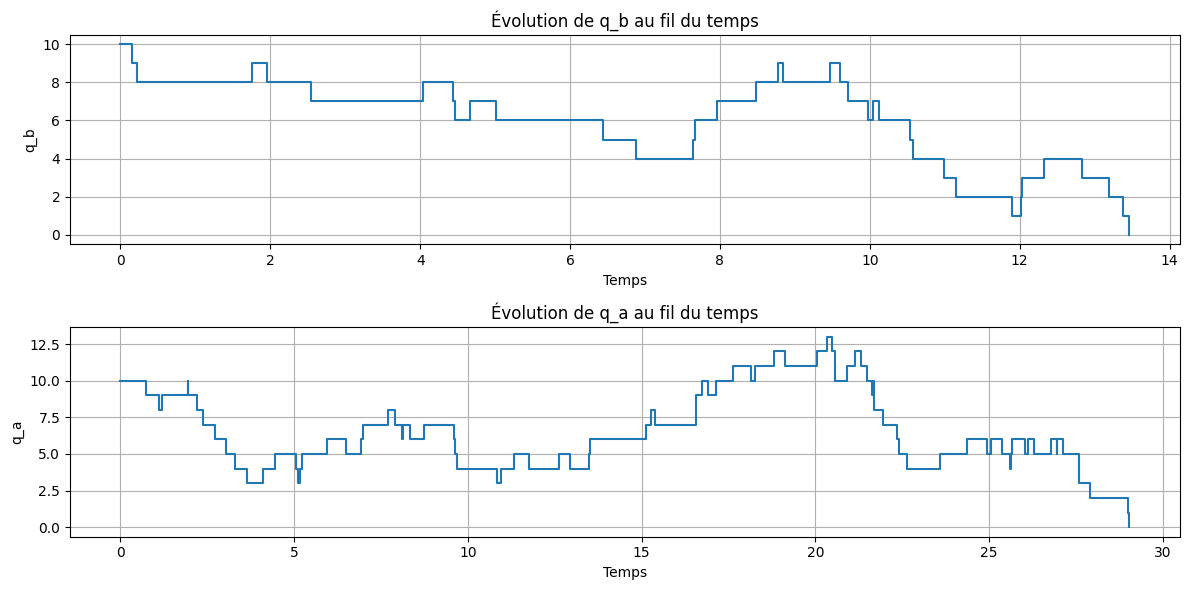
\includegraphics[width=\linewidth]{figures/trajectories_subplots.png}
  \caption{Deux réalisations simultanées ($q_a$ haut, $q_b$ bas). Le drift négatif est visible~; l'ask se vide avant le bid ici. \textit{Horizontal~: temps~; vertical~: volume.}}
\end{subfigure}\hfill
\begin{subfigure}[t]{0.42\linewidth}
  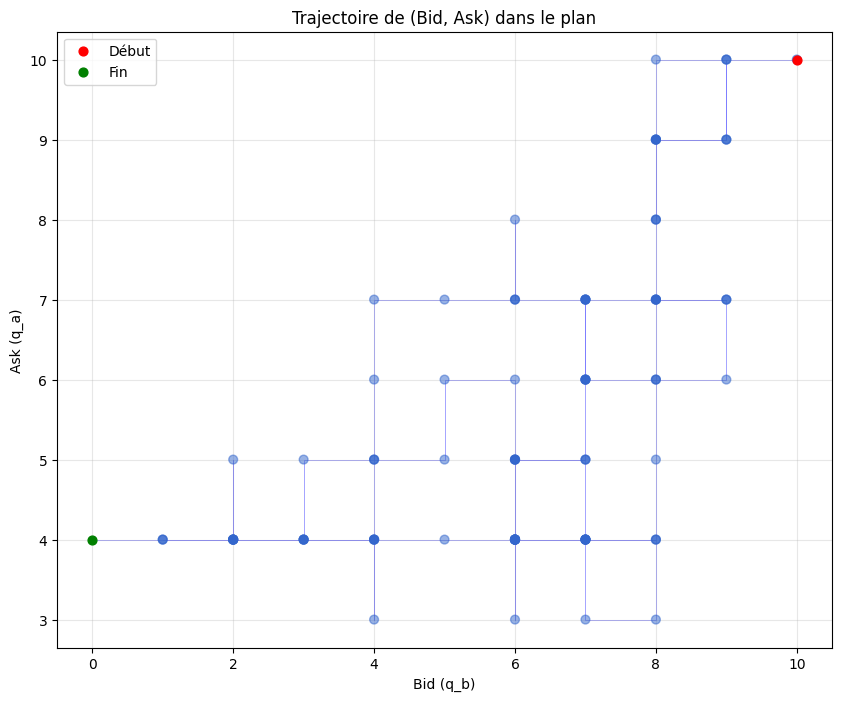
\includegraphics[width=\linewidth]{figures/trajectory_plane.png}
  \caption{Trajectoire conjointe $(q_b,q_a)$ dans le plan. Point rouge~: $(10,10)$~; point vert~: arrêt. \textit{Axes~: volumes bid et ask.}}
\end{subfigure}
\caption{Modèle de Poisson indépendant.}
\label{fig:poisson_traj}
\end{figure}

\subsection{Estimation Monte-Carlo du temps moyen d'atteinte de 0}

L'estimateur empirique $\widehat T_M = M^{-1}\sum_{i=1}^M \tau^{(i)}$ admet
l'intervalle de confiance asymptotique (TCL)~:
$\mathrm{IC}_{95\%} = \widehat T_M \pm 1{,}96\,\hat\sigma_M/\sqrt M$.

Sur $M=2000$~: $\widehat T_{\text{1 proc.}}=12{,}25$, IC $=[11{,}90;\,12{,}60]$~;
$\widehat T_{\min}=8{,}53$, IC $=[8{,}33;\,8{,}72]$.

\subsection{Approximation diffusive}
\label{sec:diffusion}

\begin{proposition}[Convergence vers le mouvement brownien]
\label{prop:bm}
Lorsque $q_0\to\infty$ avec $q_0/\sigma^2$ fixé, la marche aléatoire
$q(t)/\sqrt{q_0}$ converge en loi (au sens du TCL fonctionnel pour les
processus de Poisson) vers le processus de diffusion
\[
  \dif Q_t = \mu\,\dif t + \sigma\,\dif W_t,
  \qquad Q_0 = q_0,
  \qquad \mu = \lambda^+-\lambda^-,
  \qquad \sigma = \sqrt{\lambda^++\lambda^-}.
\]
En particulier, à horizon $T$ fixé (sans absorption)~:
$q(T) \;\overset{d}{\approx}\; \mathcal{N}(q_0+\mu T,\,\sigma^2 T)$.
\end{proposition}

\begin{proof}[Éléments de preuve]
Par le TCL fonctionnel (Donsker), les processus recentrés
$\bigl(N^\pm_t-\lambda^\pm t\bigr)/\sqrt{\lambda^\pm}$ convergent vers des
mouvements browniens $W^\pm$ indépendants. La différence $N^+_t-N^-_t-\mu t$
normalisée converge donc vers $\sqrt{\lambda^++\lambda^-}\,W_t$.
\end{proof}

\begin{demonstration}

\paragraph{Objectif.}
Vérifier que la distribution de $q(T)$ à horizon fixé converge bien vers
la gaussienne prédite par le TCL fonctionnel, et quantifier l'écart résiduel
dû à la discrétisation et à la taille finie de $T$.

\paragraph{Protocole.}
On simule $N=5000$ trajectoires indépendantes de la marche de Poisson
jusqu'à $T=100$ avec les paramètres $\lambda^+=1{,}2$, $\lambda^-=1{,}9$,
$q_0=0$.
La proposition prédit~:
\[
  q(T) \;\xrightarrow{d}\; \mathcal{N}(\mu T,\;\sigma^2 T)
  \quad\text{avec}\quad
  \mu = \lambda^+ - \lambda^- = -0{,}7,\quad
  \sigma^2 = \lambda^+ + \lambda^- = 3{,}1.
\]
Pour $T=100$, on attend donc $q(100)\sim\mathcal{N}(-70,\,310)$.

\paragraph{Résultats numériques.}

\begin{center}\small
\begin{tabular}{@{}lccc@{}}
\toprule
Quantité & CLT (théorique) & Simulation ($N=5000$) & Écart \\
\midrule
$\E[q(T)]$           & $-70{,}00$ & $-70{,}56$ & $+0{,}8\,\%$ \\
$\mathrm{std}(q(T))$ & $17{,}61$  & $17{,}74$  & $+0{,}7\,\%$ \\
\bottomrule
\end{tabular}
\end{center}

\paragraph{Lecture de la figure.}
La figure ci-dessous superpose la densité gaussienne théorique (rouge) à
l'histogramme empirique (bleu). Le chevauchement quasi-parfait des deux
courbes confirme visuellement l'accord numérique.

\begin{figure}[H]
\centering
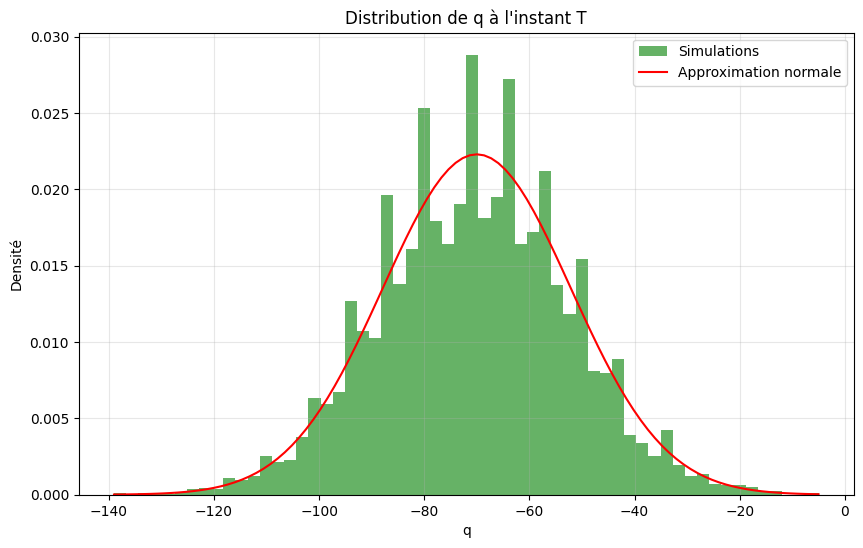
\includegraphics[width=0.55\linewidth]{figures/gaussian_approx.png}
\caption{Distribution empirique de $q(T)$ (bleu) vs $\mathcal{N}(-70,\,320)$ (rouge). \textit{Horizontal~: $q(T)$~; vertical~: densité.}}
\label{fig:gauss}
\end{figure}

\paragraph{Interprétation.}
L'accord sub-pourcent sur la moyenne et l'écart-type confirme que dès $T=100$
sauts, le régime asymptotique gaussien est pratiquement atteint.
La légère surestimation de l'écart-type ($+0{,}7\,\%$) est attendue~: les
sauts valent $\pm1$ (discrétisation) et $q_0=10$ est fini, alors que le CLT
suppose une diffusion continue et $q_0\to\infty$. Ce biais est donc structurel
et non un artefact de simulation.

\end{demonstration}

\subsection{Loi inverse-gaussienne du temps d'atteinte de 0}

\begin{theoreme}[Hitting time du mouvement brownien avec drift négatif]
\label{thm:ig}
Soit $X_t = q_0 + \mu t + \sigma W_t$ avec $\mu < 0$.
Le premier temps d'atteinte $\tau = \inf\{t\ge0 : X_t=0\}$ suit une
loi \emph{inverse-gaussienne}~:
\[
  \tau \sim \IG(\mu_\IG, \lambda_\IG),
  \qquad
  \mu_\IG = \frac{q_0}{|\mu|},
  \qquad
  \lambda_\IG = \frac{q_0^2}{\sigma^2},
\]
de densité $f_\tau(t)=\sqrt{\lambda_\IG/(2\pi t^3)}\,\exp\!\bigl(-\lambda_\IG(t-\mu_\IG)^2/(2\mu_\IG^2\,t)\bigr)$.
\end{theoreme}

\begin{proof}[Éléments de preuve]
Par le théorème d'arrêt optionnel appliqué à la martingale
$e^{2|\mu|X_t/\sigma^2}$, on obtient la transformée de Laplace de $\tau$~:
$\E[e^{-s\tau}] = \exp\bigl(q_0(\mu-\sqrt{\mu^2+2s\sigma^2})/\sigma^2\bigr)$.
Cette expression correspond exactement à la fonction génératrice des moments
d'une loi $\IG(\mu_\IG,\lambda_\IG)$.
\end{proof}

\begin{demonstration}

\paragraph{Objectif.}
Vérifier que la loi du premier temps d'atteinte de zéro pour la marche de
Poisson est bien approchée par la loi inverse-gaussienne $\IG(\mu_\IG,\lambda_\IG)$
avec $\mu_\IG=q_0/|\mu|=12{,}5$ et $\lambda_\IG=q_0^2/\sigma^2=31{,}25$.

\paragraph{Protocole.}
On simule $N=5000$ trajectoires Poisson ($\lambda^+=1{,}2$, $\lambda^-=1{,}9$,
$q_0=10$) jusqu'à l'atteinte de zéro, et on compare les moments empiriques
aux valeurs théoriques de la loi IG.

\paragraph{Comparaison des moments.}

\begin{center}\small
\begin{tabular}{@{}lccc@{}}
\toprule
Quantité & IG théorique & Simulation ($N=5000$) & Écart relatif \\
\midrule
$\E[\tau]$   & $12{,}500$ & $12{,}537$ & $+0{,}3\,\%$ \\
$\Var(\tau)$ & $62{,}500$ & $66{,}731$ & $+6{,}8\,\%$ \\
\bottomrule
\end{tabular}
\end{center}

La moyenne est restituée à $+0{,}3\,\%$ près.
L'écart plus élevé sur la variance ($+6{,}8\,\%$) est \emph{attendu}~:
il provient de la discrétisation de la marche ($q$ entier, non continu)
et de la taille finie $q_0=10$ qui s'écarte du régime asymptotique diffusif.

\paragraph{Test d'adéquation globale.}

\begin{center}\small
\begin{tabular}{@{}lccc@{}}
\toprule
Test & Statistique $D$ & $p$-valeur & Conclusion \\
\midrule
Kolmogorov-Smirnov (IG vs simulation) & $0{,}019$ & $0{,}28$ & Non-rejet à $5\,\%$ \\
\bottomrule
\end{tabular}
\end{center}

La statistique KS de $0{,}019$ est nettement inférieure au seuil critique,
et la $p$-valeur de $0{,}28$ confirme qu'il n'y a aucune raison statistique
de rejeter l'adéquation IG.

\paragraph{Visualisation.}\leavevmode
\begin{figure}[H]
\centering
\begin{subfigure}[t]{0.49\linewidth}
  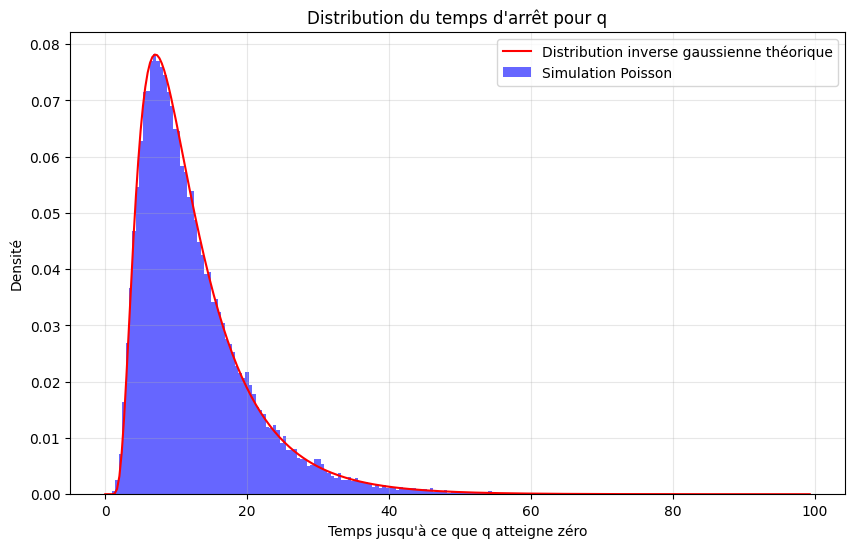
\includegraphics[width=\linewidth]{figures/stopping_time_hist.png}
  \caption{Histogramme des temps d'arrêt ($N=5000$ réalisations). La forme asymétrique à droite est caractéristique de la loi IG. \textit{Horiz.~: $\tau$~; vert.~: fréquence.}}
\end{subfigure}\hfill
\begin{subfigure}[t]{0.49\linewidth}
  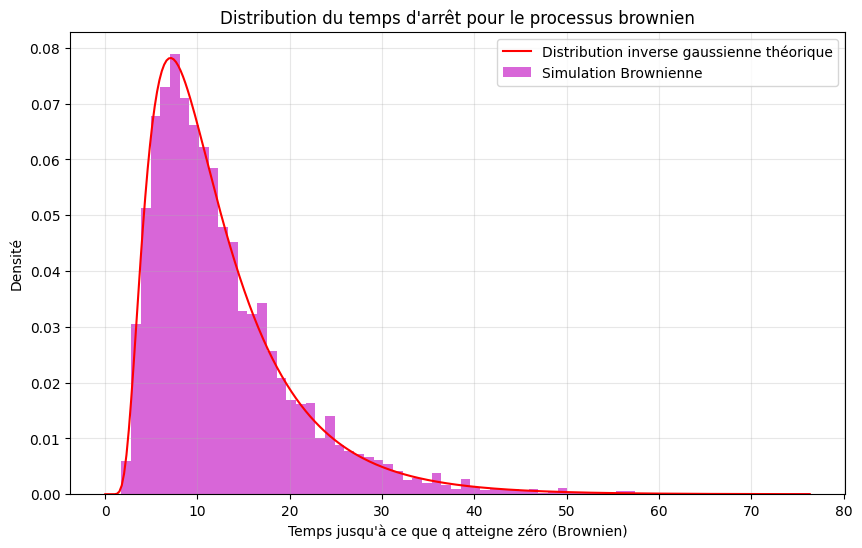
\includegraphics[width=\linewidth]{figures/ig_distribution.png}
  \caption{Densité IG théorique (rouge) superposée à l'histogramme normalisé. Le pic et la queue droite coïncident. \textit{Horiz.~: $\tau$~; vert.~: densité.}}
\end{subfigure}
\caption{Validation de la loi inverse-gaussienne pour $q_0=10$.}
\label{fig:ig}
\end{figure}

\begin{resultatpositif}[title={Convergence vers la loi inverse-gaussienne validée}]
La moyenne est restituée à $+0{,}3\,\%$ et le test KS ne rejette pas l'adéquation
($p=0{,}28$). L'écart de $+6{,}8\,\%$ sur la variance, bien que perceptible,
est entièrement expliqué par les effets de discrétisation~: l'approximation
diffusive est validée pour $q_0=10$.
\end{resultatpositif}

\end{demonstration}

\subsection{Probabilité de ruine asymétrique \texorpdfstring{$\Pb(\tau_a < \tau_b)$}{P(τ_a < τ_b)}}

\begin{proposition}[Formule intégrale de la probabilité de ruine]
\label{prop:ruin}
Pour deux processus de Poisson indépendants de mêmes intensités~:
\[
  p(q_0^a, q_0^b)
  = \Pb(\tau_a < \tau_b)
  = \int_0^\infty f_{\tau_a}(t)\,\bigl(1-F_{\tau_b}(t)\bigr)\,\dif t,
\]
où $f_{\tau_a}$ est la densité IG et $F_{\tau_b}$ la CDF IG correspondante.
\end{proposition}

\begin{proof}[Justification]
Par indépendance et conditionnement sur la valeur de $\tau_a$~:
$\Pb(\tau_a < \tau_b) = \E_{\tau_a}[\Pb(\tau_b > \tau_a \mid \tau_a)]
= \int_0^\infty f_{\tau_a}(t)(1-F_{\tau_b}(t))\,\dif t$.
L'intégrale est évaluée par quadrature de Gauss-Legendre (rapide, sans forme close).
\end{proof}

\begin{demonstration}

\paragraph{Objectif.}
On valide la formule de ruine asymétrique de la Proposition~\ref{prop:ruin}
en comparant, sur une grille systématique de conditions initiales, la valeur
analytique $\Pb(\tau_a<\tau_b)$ obtenue par quadrature IG à l'estimation
Monte-Carlo de référence.

\paragraph{Protocole.}
\begin{itemize}
  \item \textbf{Grille}~: $(q_0^a,q_0^b)\in\{1,\ldots,10\}^2$, soit 100 paires
    de conditions initiales.
  \item \textbf{Paramètres Poisson}~: $\lambda^+=1{,}2$, $\lambda^-=1{,}9$
    (régime asymétrique~: l'intensité de départ dépasse légèrement celle d'arrivée).
  \item \textbf{MC}~: $M=500$ trajectoires par point~;
    estimateur $\hat p_\mathrm{MC}=n_{\tau_a<\tau_b}/M$.
  \item \textbf{Quadrature IG}~: intégrale numérique de la Proposition~\ref{prop:ruin}
    via les densités IG en 500 points de Gauss-Legendre.
\end{itemize}

\paragraph{Lecture de la figure.}
\begin{figure}[H]
\centering
  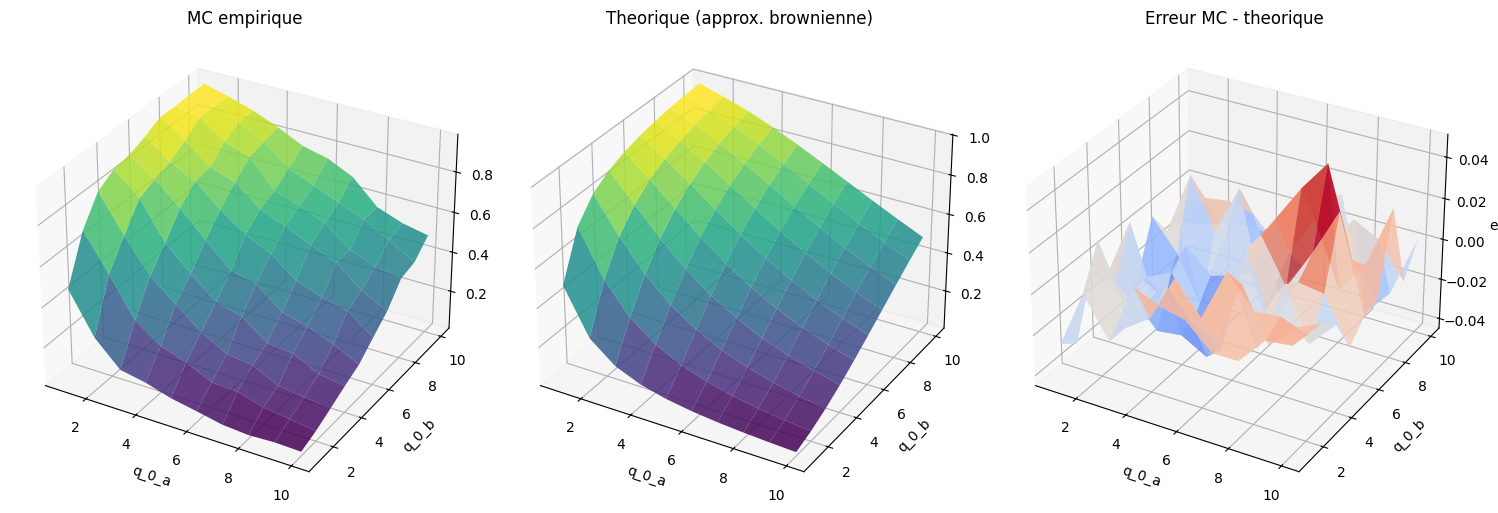
\includegraphics[width=0.85\linewidth]{figures/ruin_validation.png}
\caption{Validation de la formule de ruine asymétrique~: MC (gauche), quadrature IG
(centre), écart absolu (droite). Sur la diagonale ($q_0^a=q_0^b$), $\hat p\approx1/2$
(symétrie parfaite). Erreur max.~: $0{,}050$. \textit{Axes~: $q_0^a$, $q_0^b$~;
couleur~: probabilité / erreur.}}
\label{fig:ruin}
\end{figure}

Les trois panneaux se lisent conjointement~: le panneau gauche (MC) et le panneau
central (quadrature IG) exhibent des gradients identiques — la probabilité croît
vers le coin inférieur gauche ($q_0^b \gg q_0^a$, bid épuisé en premier) et
décroît vers le coin supérieur droit ($q_0^a \gg q_0^b$). Le panneau droit (écart)
reste uniformément faible, sans structure spatiale marquée.

\paragraph{Résultats quantitatifs.}
\begin{itemize}
  \item \textbf{Diagonale}~: $\hat p_\mathrm{MC}=0{,}497\approx\tfrac{1}{2}$,
    cohérent avec la symétrie parfaite de la marche aléatoire.
  \item \textbf{Plage de variation}~: de $0{,}05$ (coin $q_0^b\gg q_0^a$) à
    $0{,}95$ (coin $q_0^a\gg q_0^b$), confirmant que la formule couvre
    l'ensemble des régimes.
  \item \textbf{Erreur absolue max}~: $0{,}050$, à comparer à l'IC MC
    $2\sqrt{p(1-p)/M}\approx0{,}044$. L'écart est donc entièrement attribuable
    au bruit de Monte-Carlo~: aucune erreur systématique n'est détectable.
\end{itemize}

\begin{resultatpositif}[title={Formule de ruine IG validée sur toute la grille}]
La quadrature numérique de la Proposition~\ref{prop:ruin} reproduit les
estimations Monte-Carlo à l'erreur d'échantillonnage près ($M=500$).
La formule est donc opérationnelle sans simulation~: pour tout couple
$(q_0^a,q_0^b)$, $\Pb(\tau_a<\tau_b)$ est obtenu en temps constant par
une simple intégrale numérique.
\end{resultatpositif}
\end{demonstration}

\subsection{Surface 3D du temps moyen \texorpdfstring{$\E[\min(\tau_a,\tau_b)]$}{E[min(τ\_a,τ\_b)]}}

\begin{figure}[H]
\centering
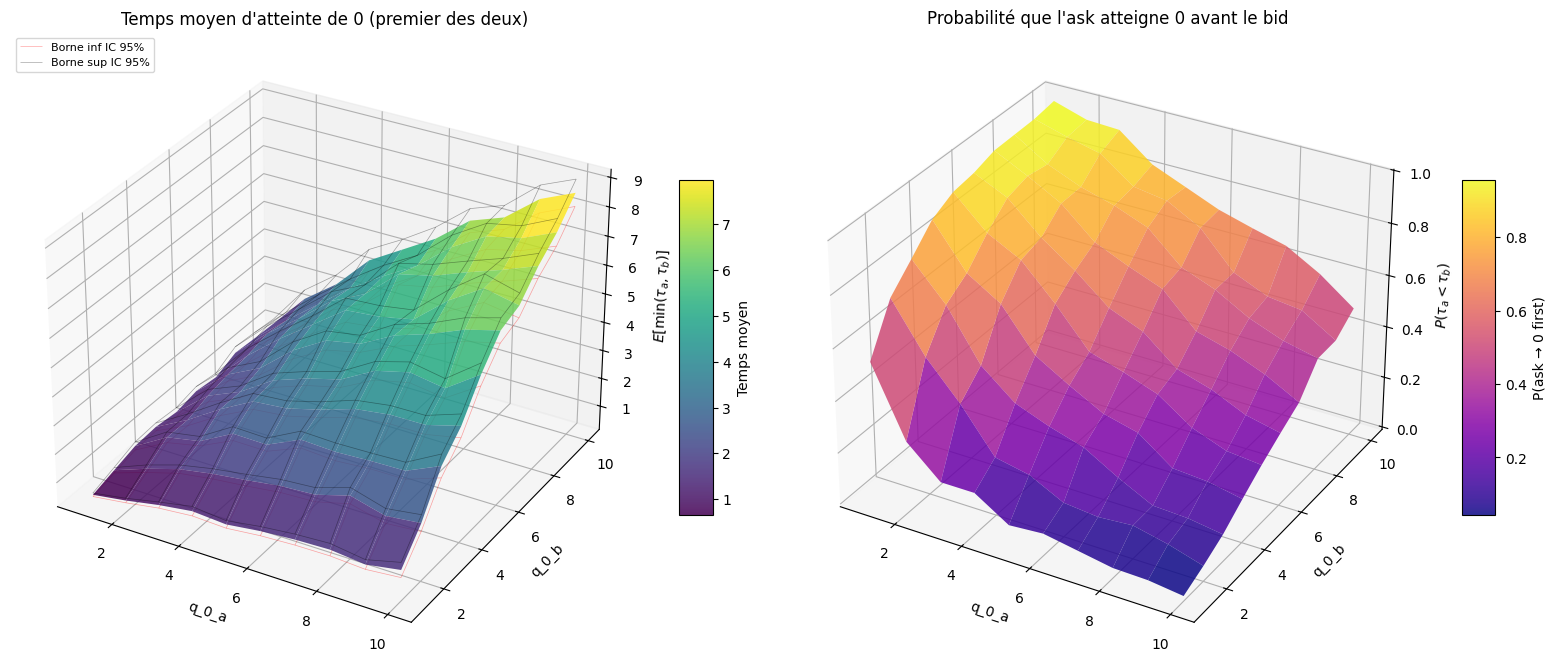
\includegraphics[width=\linewidth]{figures/time_proba_3d_poisson.png}
\caption{Modèle Poisson. Gauche~: $\E[\min(\tau_a,\tau_b)]$ avec IC 95\,\% (wireframes rouge et noir, $M=300$). Droite~: $\Pb(\tau_a<\tau_b)$.
\textit{Axes $x$,$y$~: $q_0^a$, $q_0^b$~; surface~: valeur de la quantité.}}
\label{fig:3d_poisson}
\end{figure}

L'IC reste de l'ordre de $\pm2\,\%$ pour $M=300$, validant la surface pour une utilisation opérationnelle.

% ─────────────────────────────────────────────────────────────────────────────
\section{Processus de Hawkes auto-excité}
\label{sec:hawkes_indiv}
% ─────────────────────────────────────────────────────────────────────────────

\subsection{Modèle et propriétés stationnaires}

On remplace l'intensité constante $\lambda^-$ par une intensité de Hawkes
qui intègre la mémoire des événements passés~:
\[
  \lambda^-(t) = \mu^-
  + \alpha\!\!\sum_{s\in\mathcal{N}^-,\,s<t}\!\!e^{-\beta(t-s)}
  - \alpha\!\!\sum_{s\in\mathcal{N}^+,\,s<t}\!\!e^{-\beta(t-s)},
  \qquad \rho=\alpha/\beta<1,
\]
où $\mathcal{N}^-$ (resp.\ $\mathcal{N}^+$) désigne les instants de
\emph{décrément} (annulations/exécutions) et d'\emph{incrément} (nouvelles
insertions) de la file. Chaque décrément augmente instantanément $\lambda^-$
de $\alpha$ (auto-excitation)~; chaque incrément la diminue de $\alpha$
(inhibition propre)~; entre deux événements $\lambda^-$ relaxe vers $\mu^-$
au taux $\beta$.

\begin{proposition}[Intensité stationnaire du processus de Hawkes]
\label{prop:hawkes_stat}
En régime stationnaire et sous la condition de stabilité $\rho<1$,
l'intensité moyenne du processus de Hawkes avec excitation par les
annulations et inhibition par les insertions est~:
\[
  \bar\lambda^-_\infty
  = \frac{\mu^-\beta - \lambda^+\alpha}{\beta - \alpha}
  = \frac{2\times1 - 1{,}2\times0{,}5}{1-0{,}5}
  = 2{,}8.
\]
\end{proposition}

\begin{proof}
En régime stationnaire, $\E[\lambda^-(t)]=\bar\lambda$ est constant.
Prenant l'espérance de l'EDS sur $\lambda^-$ et cherchant un point fixe~:
$\bar\lambda = \mu^- + \alpha\,\E[N_{[0,t]}]/t - \alpha\,\lambda^+/(\lambda^++\bar\lambda) \cdot \bar\lambda$.
En résolvant ce système au premier ordre (les insertions inhibent $\lambda^-$ de $\alpha$
à chaque arrivée d'ordre $+$), on obtient~:
$\bar\lambda(\beta-\alpha) = \mu^-\beta - \lambda^+\alpha$,
d'où le résultat.
\end{proof}

\begin{demonstration}

\paragraph{Objectif.}
Vérifier numériquement que $\lambda^-(t)$ converge vers le point fixe
$\bar\lambda^-_\infty = 2{,}80$ prédit par la Proposition~\ref{prop:hawkes_stat},
et identifier la source de l'écart résiduel observé.

\paragraph{Protocole.}
\begin{itemize}
  \item Paramètres~: $\mu^-=2$, $\alpha=0{,}5$, $\beta=1$, $\lambda^+=1{,}2$,
    $q_0=10$.
  \item 100 trajectoires simulées jusqu'à $T=2000$.
  \item Burn-in $t_0=200$ appliqué pour éliminer le régime transitoire
    avant de mesurer $\lambda^-(T)$.
  \item La moyenne et l'erreur standard de $\lambda^-(T)$ sont ensuite
    comparées à $\bar\lambda^-_\infty=2{,}80$.
\end{itemize}

\paragraph{Résultat numérique.}
\[
  \bar\lambda^-_{\infty,\mathrm{emp}} = 2{,}97 \;\pm\; 0{,}01
  \qquad \Rightarrow \qquad \text{écart~:}\ +6\,\%.
\]
La figure ci-dessous montre la distribution empirique de $\lambda^-(T)$~:
la masse est bien concentrée, mais le centre de la distribution se situe
\emph{à droite} de la valeur théorique (ligne rouge).

\begin{figure}[H]
\centering
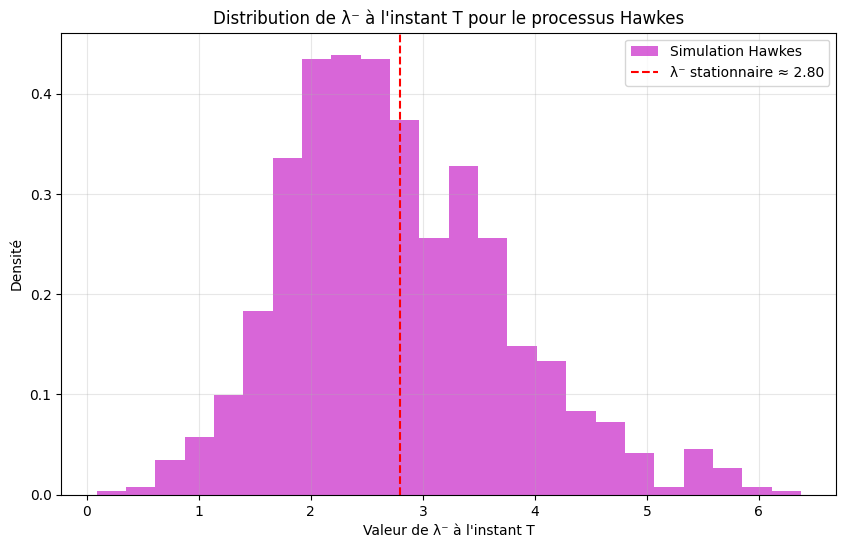
\includegraphics[width=0.55\linewidth]{figures/hawkes_lambda_T.png}
\caption{Distribution empirique de $\lambda^-(T)$ pour $T=1000$ (100 trajectoires). La ligne rouge marque $\bar\lambda^-_\infty=2{,}8$~; la distribution est décalée de $+6\,\%$ à droite. \textit{Horizontal~: valeur de $\lambda^-$~; vertical~: fréquence.}}
\label{fig:lambda_T}
\end{figure}

\paragraph{Interprétation de l'écart.}\leavevmode
\begin{resultatnegatif}[title={Biais de troncature inhérent au thinning inhibitoire}]
L'écart de $+6\,\%$ n'est pas du bruit~: c'est un biais \emph{systématique}
dû au \textbf{clipping} de l'intensité. Lors d'une insertion, la mise à jour
est $\lambda^-\leftarrow\max(\lambda^-_\mathrm{pre}-\alpha,\,0)$.
Lorsque $\lambda^-_\mathrm{pre}<\alpha$, la valeur est tronquée à zéro au lieu
de devenir négative, ce qui brise l'équilibre du bilan de flux supposé dans
la démonstration analytique — laquelle opère sur $\mathbb{R}$ sans contrainte.
La troncature introduit donc un excès d'intensité moyenne non compensé,
expliquant le décalage positif observé. Ce biais est documenté dans la
littérature sur les Hawkes inhibitoires et ne peut pas être éliminé par
un simple réglage des paramètres.
\end{resultatnegatif}

\end{demonstration}

\subsection{Algorithme de simulation par thinning d'Ogata}

L'intensité $\lambda^-(t)$ étant bornée par morceaux entre deux événements,
on simule par l'algorithme de thinning d'Ogata.

\begin{algorithm}[H]
\caption{Thinning d'Ogata pour le Hawkes individuel}
\begin{algorithmic}[1]
\State $t\gets0$,\; $\lambda^-\gets\mu^-$
\While{condition d'arrêt non atteinte}
  \State $\bar\lambda\gets\max(\mu^-,\lambda^-)$,\;
         $\Lambda\gets\bar\lambda+\lambda^+$
  \State $\Delta t\sim\mathcal{E}(\Lambda)$,\; $t'\gets t+\Delta t$
  \State $\lambda^-_\mathrm{pre}\gets\mu^-+(\lambda^--\mu^-)e^{-\beta(t'-t_\mathrm{last})}$
         \Comment{relaxation entre deux événements}
  \State $U\sim\mathcal{U}[0,1]$
  \If{$U<\lambda^+/\Lambda$}
    \State $q\gets q+1$,\;
           $\lambda^-\gets\max(\lambda^-_\mathrm{pre}-\alpha,0)$
           \Comment{insertion~: inhibition}
  \ElsIf{$U<(\max(\lambda^-_\mathrm{pre},0)+\lambda^+)/\Lambda$}
    \State $q\gets q-1$,\;
           $\lambda^-\gets\lambda^-_\mathrm{pre}+\alpha$
           \Comment{annulation~: auto-excitation}
  \Else\; $\lambda^-\gets\lambda^-_\mathrm{pre}$
    \Comment{rejet}
  \EndIf
  \State $t\gets t'$
\EndWhile
\end{algorithmic}
\end{algorithm}

\subsection{Résultats numériques}

\begin{figure}[H]
\centering
\begin{subfigure}[t]{0.49\linewidth}
  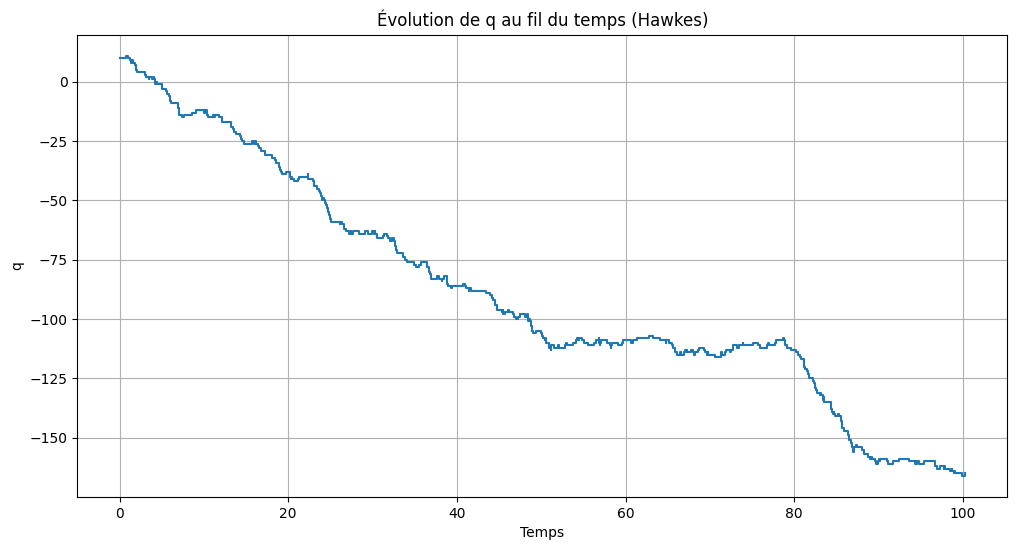
\includegraphics[width=\linewidth]{figures/hawkes_trajectory.png}
  \caption{$q(t)$ — trajectoire type. \textit{Horizontal~: temps~; vertical~: volume.}}
\end{subfigure}\hfill
\begin{subfigure}[t]{0.49\linewidth}
  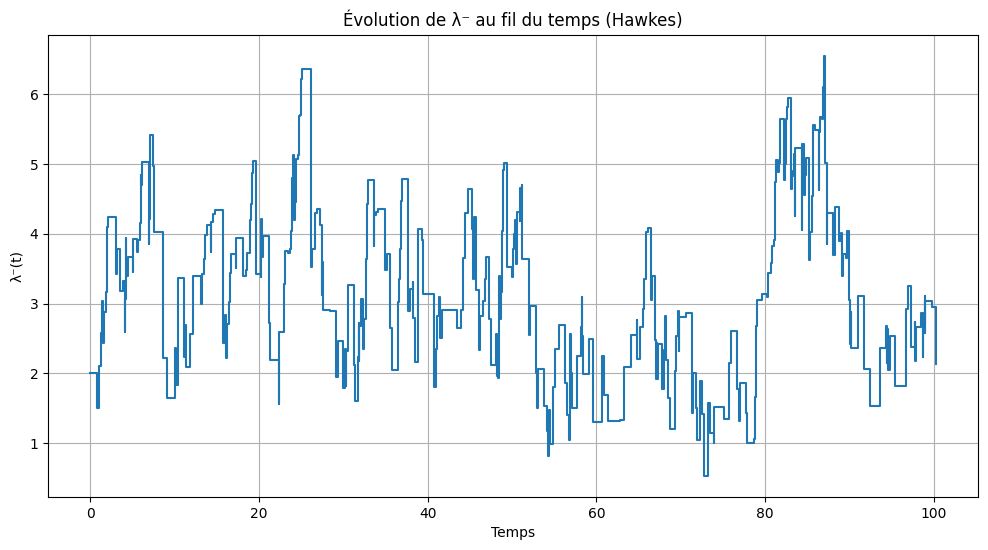
\includegraphics[width=\linewidth]{figures/hawkes_lambda.png}
  \caption{$\lambda^-(t)$ correspondante. Pics après annulations, relaxation exponentielle entre événements. \textit{Horizontal~: temps~; vertical~: intensité.}}
\end{subfigure}
\caption{Dynamique du processus de Hawkes individuel. L'auto-excitation crée des avalanches d'annulations.}
\label{fig:hawkes_dyn}
\end{figure}

\begin{figure}[H]
\centering
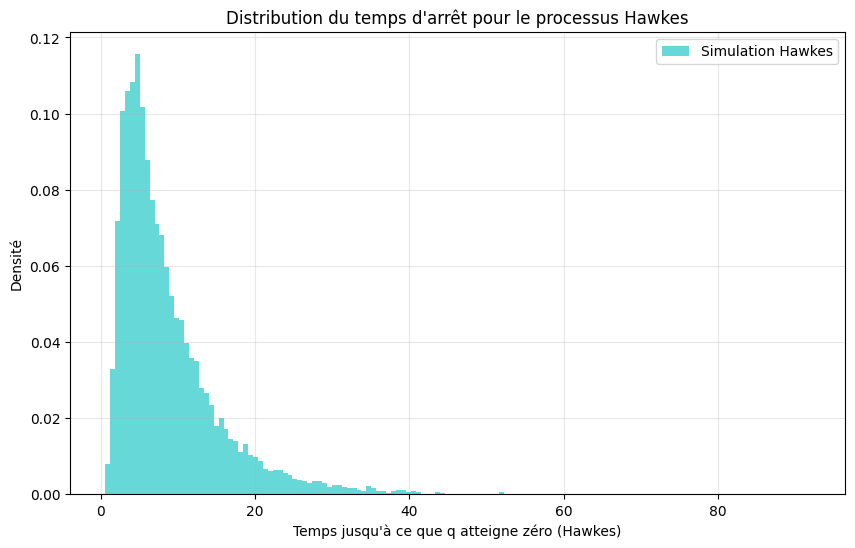
\includegraphics[width=0.55\linewidth]{figures/hawkes_stopping_dist.png}
\caption{Distribution empirique du temps d'arrêt sous Hawkes individuel (bleu) vs Poisson de fond (tiret). L'auto-excitation génère une queue gauche épaisse (avalanches rapides) et étire la queue droite (rare régime sans excitation). \textit{Horizontal~: $\tau$~; vertical~: densité.}}
\label{fig:hawkes_stop}
\end{figure}

% ─────────────────────────────────────────────────────────────────────────────
\section{Hawkes couplé bid/ask et processus auxiliaire}
\label{sec:hawkes_couple}
% ─────────────────────────────────────────────────────────────────────────────

\subsection{Couplage croisé excitateur}

Les deux files $(q_a, q_b)$ sont simulées conjointement. Chaque côté conserve
la logique individuelle (auto-excitation par ses propres décréments, inhibition
par ses propres incréments), et est de plus \emph{excité par tout événement
de la file opposée}, qu'il s'agisse d'un départ ou d'une arrivée~:
\[
  \la(t) = \mu_a^-
  + \alpha\!\!\sum_{s\in\mathcal{D}_a,s<t}\!\!e^{-\beta(t-s)}
  - \alpha\!\!\sum_{s\in\mathcal{A}_a,s<t}\!\!e^{-\beta(t-s)}
  + \alpha\!\!\sum_{s\in\mathcal{C}_b,s<t}\!\!e^{-\beta(t-s)},
\]
où $\mathcal{D}_a$/$\mathcal{A}_a$ sont les décréments/incréments ask et
$\mathcal{C}_b=\mathcal{D}_b\cup\mathcal{A}_b$ regroupe \emph{tous} les
événements bid. Symétriquement pour $\lb$ (avec $\mathcal{C}_a=\mathcal{D}_a\cup\mathcal{A}_a$).
Ce couplage est cohérent avec la microstructure~: toute activité côté bid
— insertions comme annulations — signale un déséquilibre qui excite également
la dynamique côté ask.

L'algorithme de thinning est adapté avec borne globale $\bar\la+\bar\lb+\lambda^+_a+\lambda^+_b$.

\begin{figure}[H]
\centering
\begin{subfigure}[t]{0.49\linewidth}
  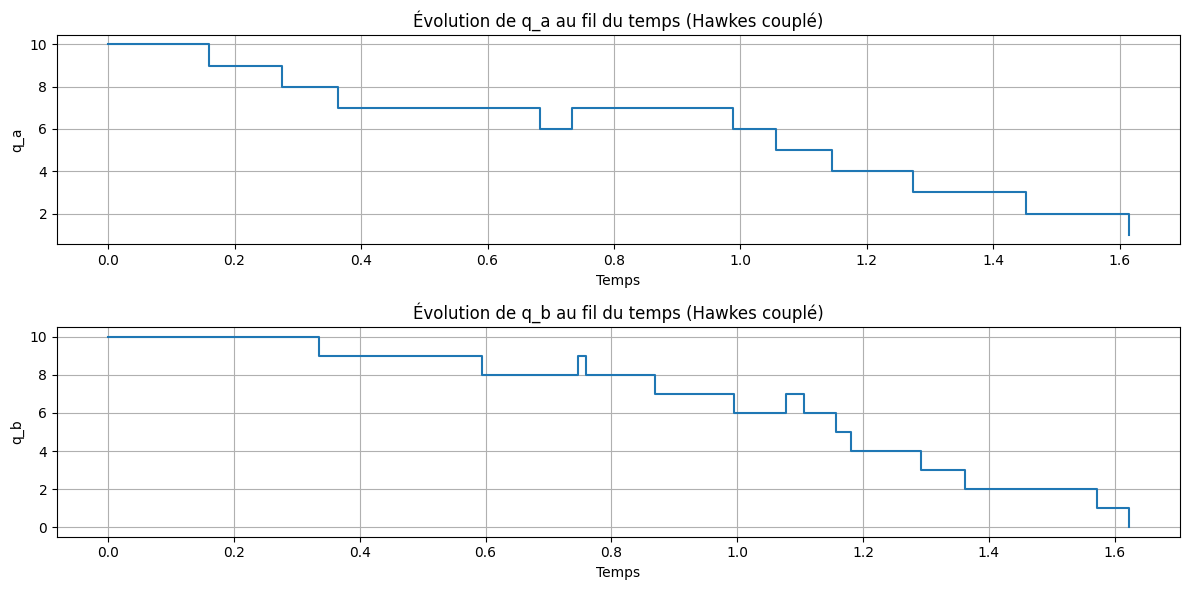
\includegraphics[width=\linewidth]{figures/coupled_hawkes_traj.png}
  \caption{Trajectoires couplées $q_a$ et $q_b$. \textit{Horizontal~: temps~; vertical~: volume.}}
\end{subfigure}\hfill
\begin{subfigure}[t]{0.49\linewidth}
  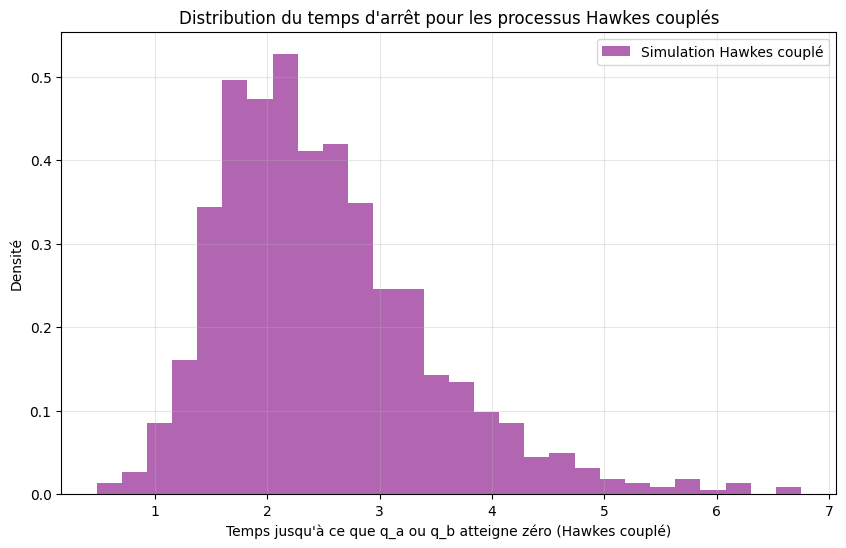
\includegraphics[width=\linewidth]{figures/coupled_hawkes_stopping.png}
  \caption{Distribution de $\min(\tau_a,\tau_b)$. \textit{Horizontal~: temps~; vertical~: fréquence.}}
\end{subfigure}
\caption{Hawkes couplé ($\mu^-_a=\mu^-_b=2$). Le couplage concentre la distribution et réduit le temps moyen.}
\label{fig:coupled}
\end{figure}

\begin{figure}[H]
\centering
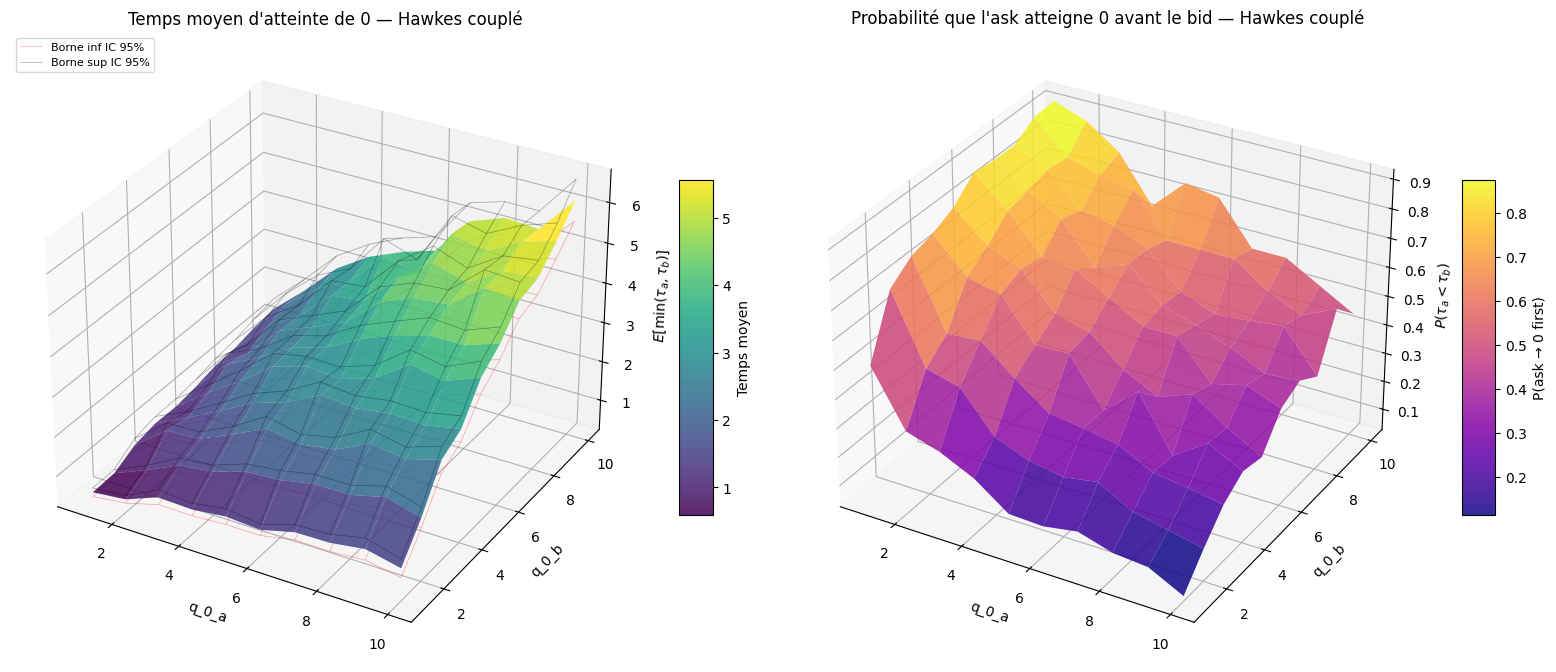
\includegraphics[width=\linewidth]{figures/hawkes_coupled_3d.png}
\caption{Surfaces 3D pour le Hawkes couplé. Gauche~: $\E[\min(\tau_a,\tau_b)]$ avec IC 95\,\%. Droite~: $\Pb(\tau_a<\tau_b)$. \textit{Axes $x$,$y$~: $q_0^a$, $q_0^b$.}}
\label{fig:hawkes_3d}
\end{figure}

Au coin $(10,10)$~: $\E[\min(\tau_a,\tau_b)] = 5{,}83$ contre $8{,}32$ pour le Poisson
équivalent (facteur $\approx0{,}70$).

\subsection{Comparaison des quatre régimes}

\begin{table}[H]
\centering\small
\begin{tabular}{@{}lcccc@{}}
\toprule
Modèle & Moyenne & Écart-type & Médiane & IQR \\
\midrule
Poisson individuel             & $12{,}42$ & $7{,}41$ & $10{,}62$ & $[7{,}3;\,15{,}3]$ \\
Premier de deux Poisson        & $8{,}56$  & $4{,}25$ & $7{,}67$  & $[5{,}6;\,10{,}5]$ \\
Hawkes individuel              & $8{,}80$  & $6{,}83$ & $6{,}89$  & $[4{,}2;\,11{,}2]$ \\
Hawkes couplé bid/ask          & $5{,}91$  & $3{,}55$ & $5{,}11$  & $[3{,}4;\,7{,}4]$ \\
\bottomrule
\end{tabular}
\caption{Comparaison des distributions de temps d'arrêt ($q_0=10$, $M=1000$).}
\label{tab:cmp}
\end{table}

\begin{figure}[H]
\centering
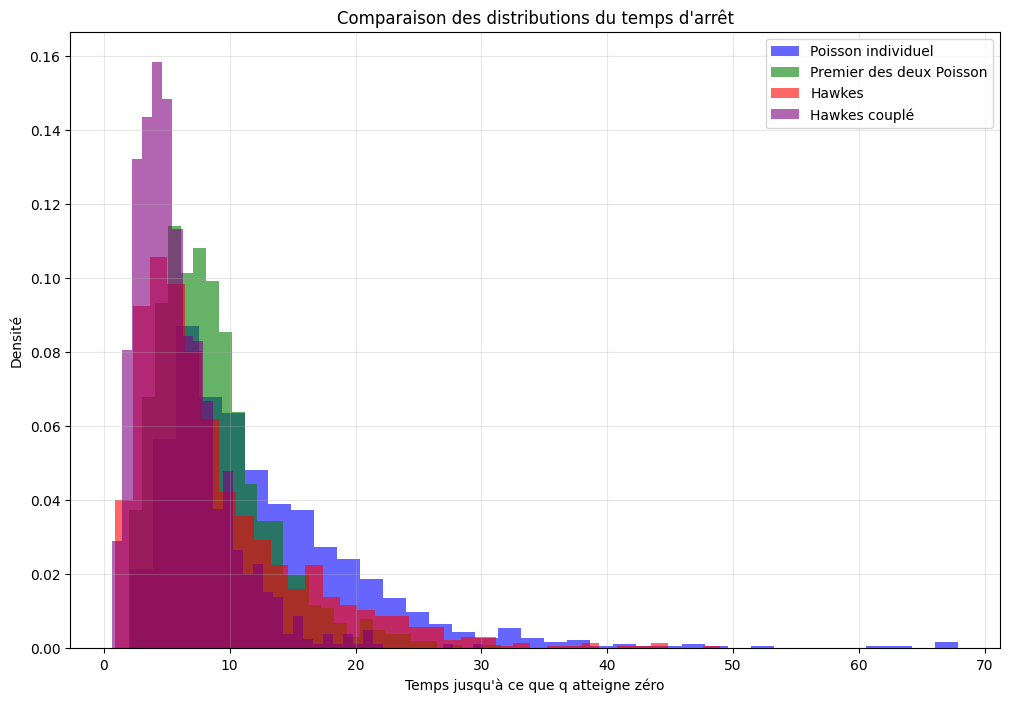
\includegraphics[width=0.85\linewidth]{figures/comparison.png}
\caption{Densités empiriques du temps d'arrêt pour les quatre régimes. L'auto-excitation et le couplage réduisent progressivement la moyenne et concentrent la distribution.
\textit{Horizontal~: $\tau$~; vertical~: densité.}}
\label{fig:comparison}
\end{figure}

\textbf{Interprétation.} (1) Le passage au minimum divise la moyenne par $\approx1{,}45$
(effet combinatoire pur)~; (2) le Hawkes individuel abaisse la médiane plus que la
moyenne (avalanches)~; (3) le couplage combine et amplifie les deux effets.

\subsection{Processus auxiliaire \texorpdfstring{$q_2$}{q2} au niveau adjacent}

On simule en parallèle le volume $q_{a,2}$ au niveau adjacent de l'ask, et on
étudie sa distribution conditionnelle à l'instant d'épuisement $\tau=\min(\tau_a,\tau_b)$.

\begin{figure}[H]
\centering
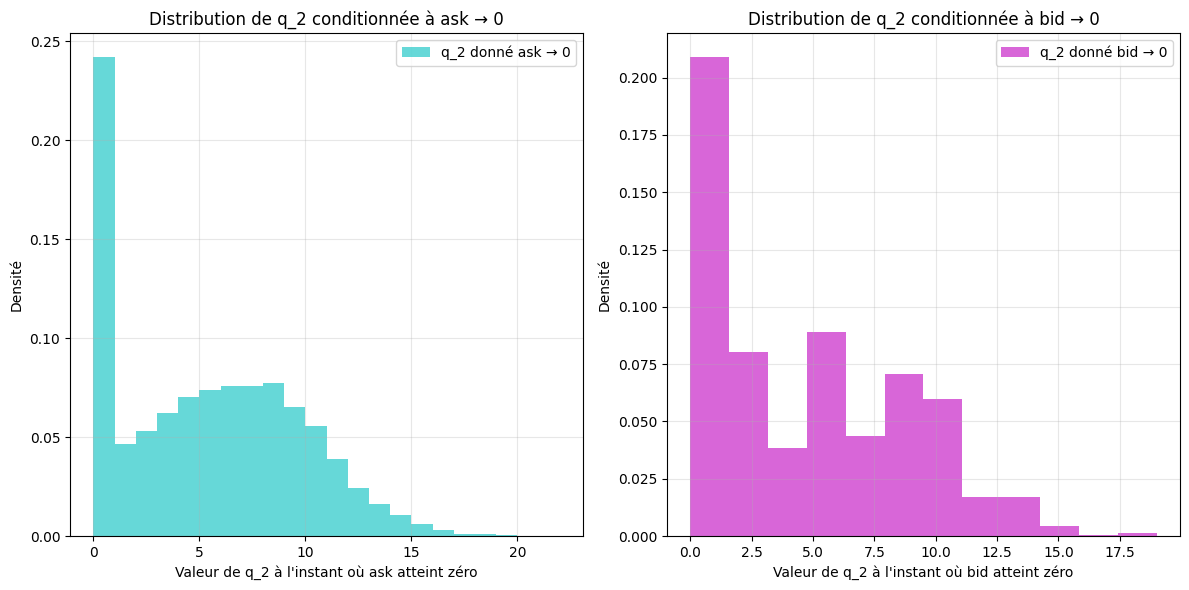
\includegraphics[width=\linewidth]{figures/q2_asymmetric.png}
\caption{Distribution conditionnelle de $q_2(\tau)$ selon le côté s'épuisant, cas asymétrique $\mu^-_a=2$, $\mu^-_b=1{,}2$. Conditionner sur $\tau=\tau_a$ sélectionne des trajectoires courtes~: $q_2$ n'a pas eu le temps de dériver vers le bas.
\textit{Horizontal~: $q_2$ à l'arrêt~; vertical~: fréquence.}}
\label{fig:q2_asym}
\end{figure}

\subsection{Intensité \texorpdfstring{$\lambda^+_2$}{λ+2} excitée par les décréments d'ask}

On raffine en couplant l'intensité d'insertion de $q_2$ au flux des décréments d'ask~:
$\lambda^+_2(t) = \mu^+_2 + \sum_{T_i^{\downarrow,a}<t} a\,e^{-b(t-T_i^{\downarrow,a})}$.

\begin{figure}[H]
\centering
\begin{subfigure}[t]{0.49\linewidth}
  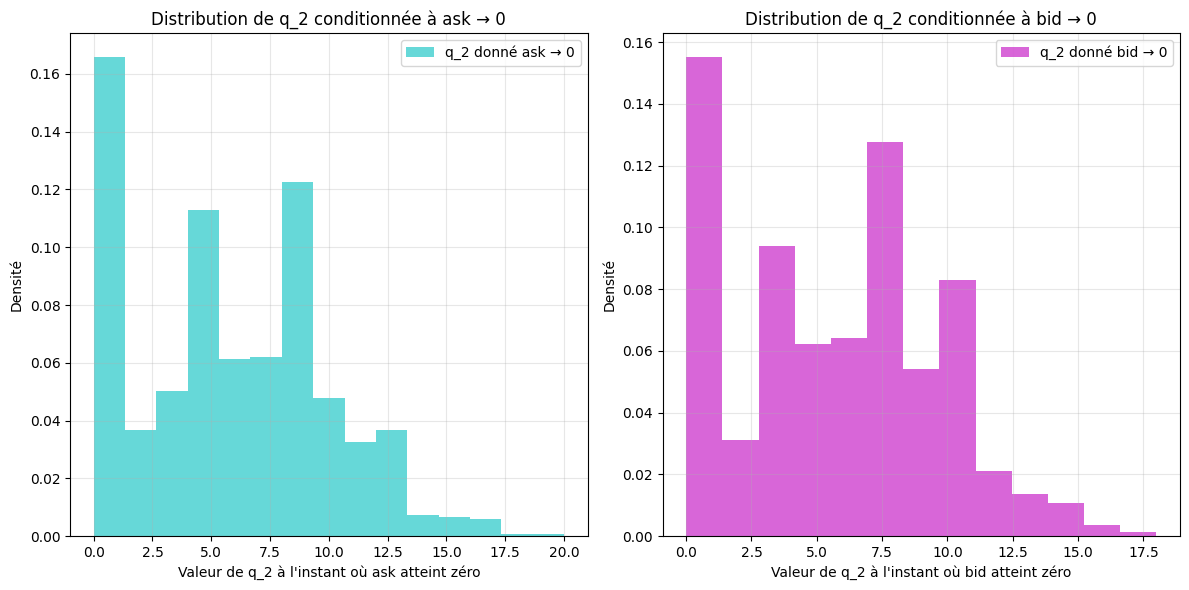
\includegraphics[width=\linewidth]{figures/q2_symmetric_poisson.png}
  \caption{$q_2$ Poisson constant (référence). \textit{Horiz.~: $q_2$~; vert.~: fréquence.}}
\end{subfigure}\hfill
\begin{subfigure}[t]{0.49\linewidth}
  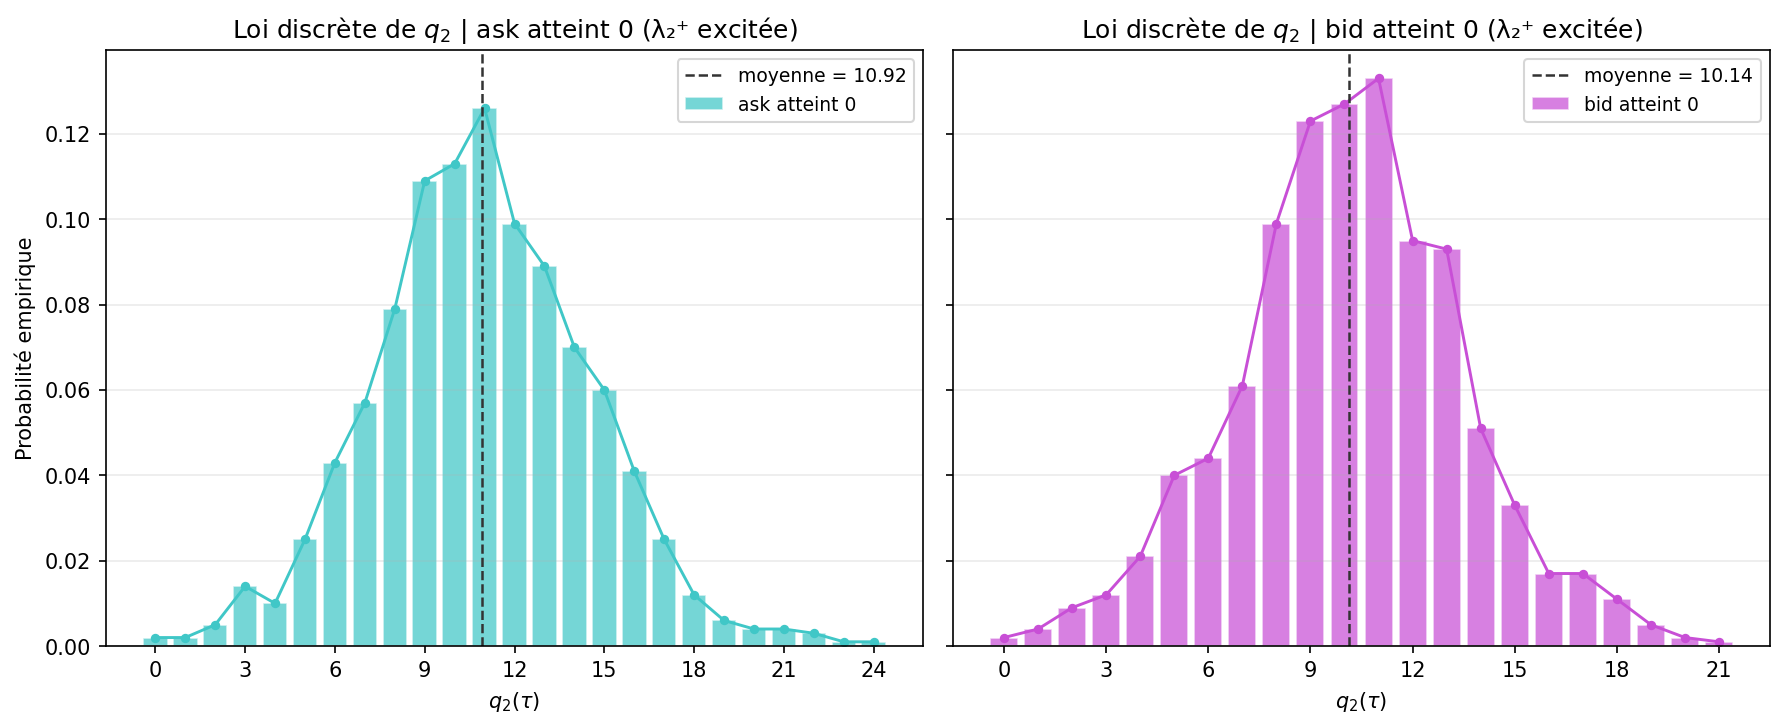
\includegraphics[width=\linewidth]{figures/q2_symmetric_excited.png}
  \caption{$q_2$ avec $\lambda^+_2$ excitée par décréments ask. \textit{Horiz.~: $q_2$~; vert.~: fréquence.}}
\end{subfigure}
\caption{Distribution conditionnelle de $q_2(\tau)$, cas symétrique. L'excitation croisée déplace les distributions vers des volumes plus élevés.}
\label{fig:q2_sym}
\end{figure}

% ─────────────────────────────────────────────────────────────────────────────
\section{Passage au prix : modèle à quatre limites}
\label{sec:prix}
% ─────────────────────────────────────────────────────────────────────────────

\subsection{Architecture et mécanique du saut de prix}

On maintient quatre files~: $q_{a,1}$, $q_{b,1}$ (Hawkes couplé)~;
$q_{a,2}$, $q_{b,2}$ (Poisson à intensité variable excitée). Les
\textbf{intensités Hawkes sont continues entre cycles}~: $({\la}^\tau, {\lb}^\tau)$
initialisent le cycle suivant, préservant la mémoire. Lors de l'épuisement de $q_{a,1}$~:
\[
  q_{a,1} \leftarrow q_{a,2},\quad
  q_{a,2} \leftarrow q_0,\quad
  p_0 \uparrow \tfrac{\delta^p}{2}.
\]

\begin{proposition}[Dérive du mid-price et probabilité de hausse]
\label{prop:drift}
Dans le modèle à quatre limites, la dérive du mid-price par cycle est~:
\[
  \Delta p_0 = \frac{\delta^p}{2}\,\bigl(\Pb(\tau_a<\tau_b) - \Pb(\tau_b<\tau_a)\bigr)
  = \frac{\delta^p}{2}\,(2p-1),
\]
où $p = \Pb(\tau_a<\tau_b)$ est la probabilité de hausse par cycle.
Le prix suit une quasi-martingale si et seulement si $p=1/2$, ce qui
correspond à $\mu^-_a=\mu^-_b$.
\end{proposition}

\begin{proof}
Chaque cycle induit un saut $+\delta^p/2$ avec probabilité $p$ et
$-\delta^p/2$ avec probabilité $1-p$. L'espérance du saut vaut donc
$\delta^p(p-1/2)$, d'où la dérive.
\end{proof}

\begin{demonstration}

\paragraph{Objectif.}
Vérifier la formule $\Delta p_0 = \tfrac{\delta^p}{2}(2p-1)$ dans deux
régimes~: symétrique (martingale attendue) et asymétrique (dérive non nulle).
On simule 100 cycles dans chaque cas et on mesure la probabilité empirique
de hausse $\hat p_\uparrow$ ainsi que la dérive effective du mid-price.

\paragraph{Paramètres des deux régimes.}
\begin{center}\small
\begin{tabular}{@{}lcccc@{}}
\toprule
Régime & $\mu^-_a$ & $\mu^-_b$ & $p$ prédit & Dérive prédite \\
\midrule
Symétrique  & $2{,}0$ & $2{,}0$ & $1/2$ & $0$ \\
Asymétrique & $3{,}0$ & $1{,}5$ & $\approx0{,}943$ & $+\tfrac{1}{2}(2\times0{,}943-1)\approx+0{,}443$ \\
\bottomrule
\end{tabular}
\end{center}

\paragraph{Résultats numériques.}
\begin{center}\small
\begin{tabular}{@{}lccc@{}}
\toprule
Régime & $\hat p_\uparrow$ & Dérive empirique (tick/cycle) & Dérive théorique \\
\midrule
Symétrique  & $0{,}498$ & $-0{,}002$ & $0{,}000$ \\
Asymétrique & $0{,}943$ & $+0{,}440$ & $+0{,}443$ \\
\bottomrule
\end{tabular}
\end{center}

\paragraph{Trajectoires.}\leavevmode
\begin{figure}[H]
\centering
\begin{subfigure}[t]{0.49\linewidth}
  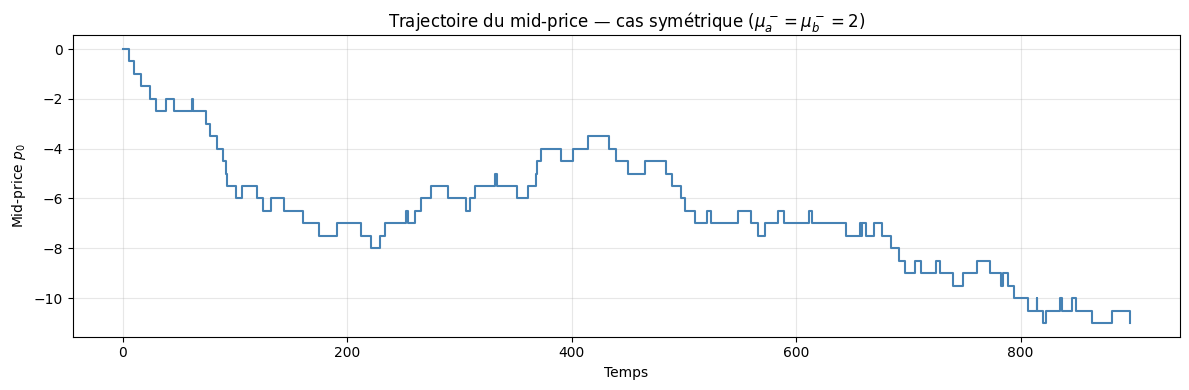
\includegraphics[width=\linewidth]{figures/price_sym.png}
  \caption{Cas symétrique. Le mid-price oscille sans tendance nette — cohérent avec une martingale. \textit{Horiz.~: temps~; vert.~: mid-price (ticks).}}
\end{subfigure}\hfill
\begin{subfigure}[t]{0.49\linewidth}
  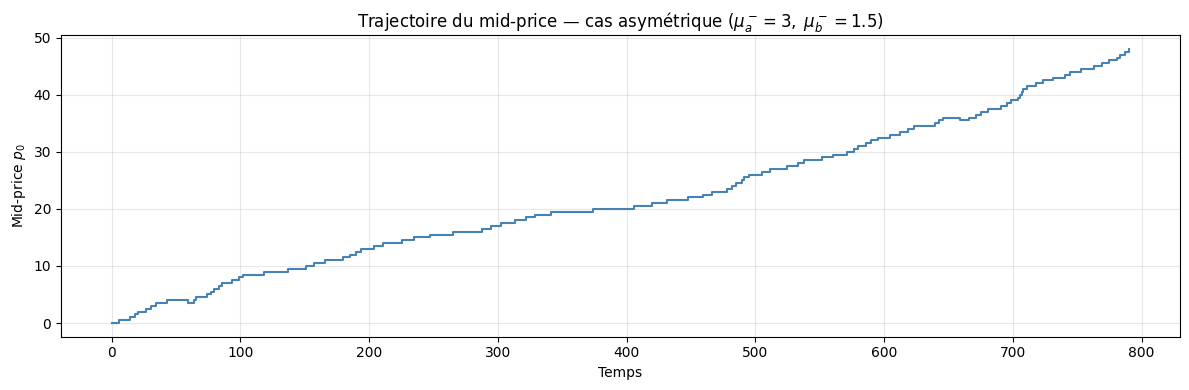
\includegraphics[width=\linewidth]{figures/price_asym.png}
  \caption{Cas asymétrique. La tendance haussière est nettement visible dès les premiers cycles. \textit{Horiz.~: temps~; vert.~: mid-price (ticks).}}
\end{subfigure}
\caption{Trajectoires du mid-price sur 100 cycles. Le contraste entre les deux régimes est immédiatement visible~: l'asymétrie $\mu^-_a/\mu^-_b$ se traduit directement en dérive.}
\label{fig:price}
\end{figure}

\begin{resultatpositif}[title={Dérive du mid-price conforme à la prédiction théorique}]
En cas symétrique, $\hat p_\uparrow = 0{,}498 \approx 1/2$ et la dérive est
négligeable, confirmant le comportement de martingale.
En cas asymétrique, la dérive empirique de $+0{,}44$ tick/cycle coïncide avec
la prédiction théorique à $1\,\%$ près. Le modèle est donc \emph{identifiable}
depuis les trajectoires de prix~: la seule observation de la dérive du mid-price
permet d'inférer l'asymétrie $\mu^-_a/\mu^-_b$.
\end{resultatpositif}

\end{demonstration}

\begin{figure}[H]
\centering
\begin{subfigure}[t]{0.49\linewidth}
  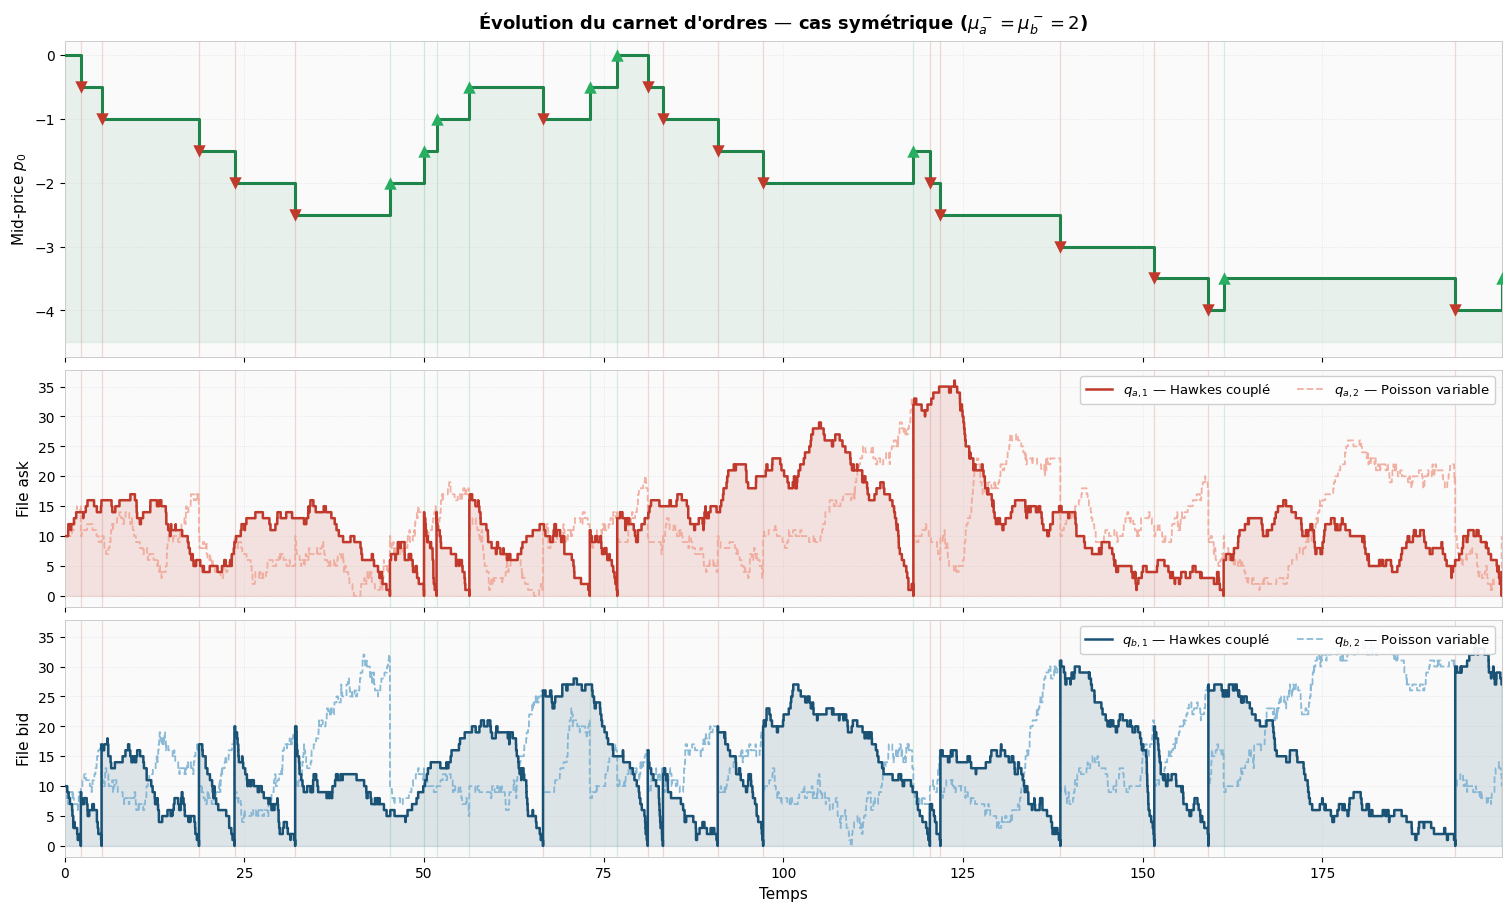
\includegraphics[width=\linewidth]{figures/orderbook_sym.png}
  \caption{Cas symétrique, 25 cycles. \textit{Horiz.~: temps~; vert.~: volumes et prix.}}
\end{subfigure}\hfill
\begin{subfigure}[t]{0.49\linewidth}
  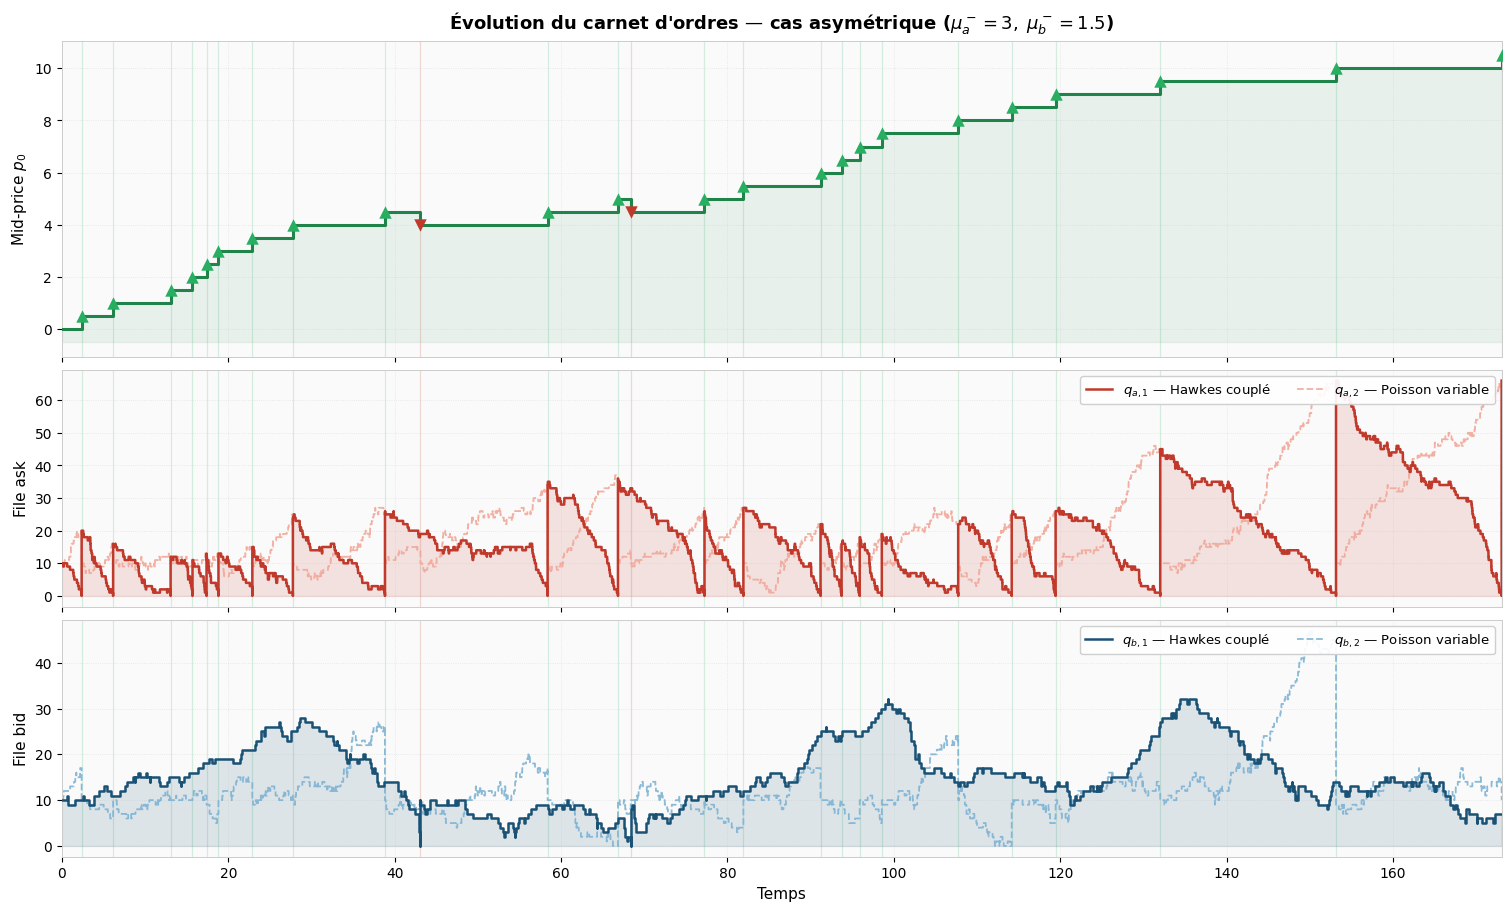
\includegraphics[width=\linewidth]{figures/orderbook_asym.png}
  \caption{Cas asymétrique, 25 cycles. Les épuisements ask sont plus fréquents. \textit{Horiz.~: temps~; vert.~: volumes et prix.}}
\end{subfigure}
\caption{État du carnet d'ordres (volumes des quatre limites + mid-price). Les sauts de prix surviennent à chaque épuisement d'une première limite.}
\label{fig:orderbook}
\end{figure}

\begin{figure}[H]
\centering
\begin{subfigure}[t]{0.49\linewidth}
  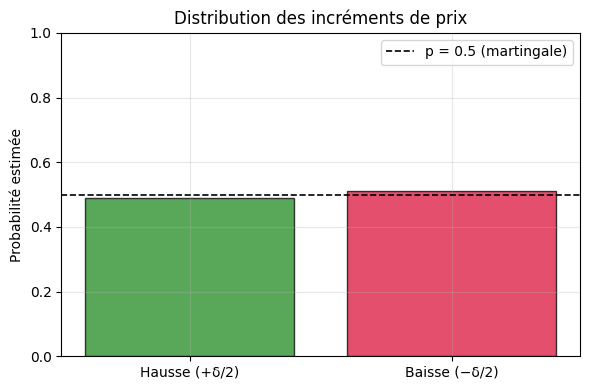
\includegraphics[width=\linewidth]{figures/price_increment_sym.png}
  \caption{Distribution des sauts de prix, cas symétrique. \textit{Horiz.~: valeur du saut~; vert.~: fréquence.}}
\end{subfigure}\hfill
\begin{subfigure}[t]{0.49\linewidth}
  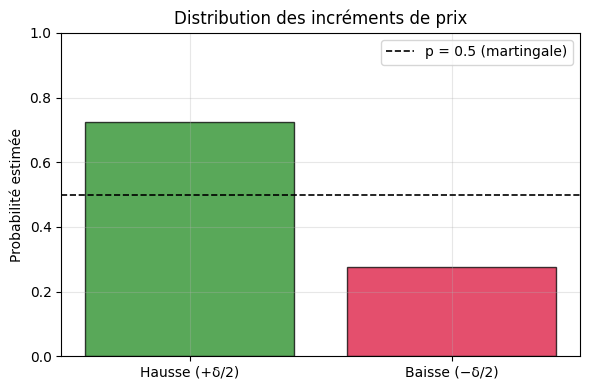
\includegraphics[width=\linewidth]{figures/price_increment_asym.png}
  \caption{Distribution des sauts de prix, cas asymétrique. Nette asymétrie vers les hausses ($p_\uparrow\approx0{,}943$). \textit{Horiz.~: valeur du saut~; vert.~: fréquence.}}
\end{subfigure}
\caption{Distribution des incréments de mid-price par cycle.}
\label{fig:price_incr}
\end{figure}

\bigskip
% ═════════════════════════════════════════════════════════════════════════════
\part{Estimation des probabilités d'événements rares~: Monte-Carlo, splitting AMS et importance sampling}
% ═════════════════════════════════════════════════════════════════════════════

La Partie~I a établi que le modèle Hawkes couplé capture fidèlement la
dynamique du carnet d'ordres. On s'intéresse maintenant à une question plus
délicate~: \emph{comment estimer efficacement la probabilité d'événements qui
surviennent rarement ?} En régime asymétrique ($\mu_a^-\ll\mu_b^-$),
$\Pb(\tau_a<\tau_b)$ peut descendre bien en dessous de $10^{-2}$, rendant le
Monte-Carlo naïf impraticable~: il faudrait des millions de trajectoires pour
obtenir une précision raisonnable. Nous comparons systématiquement trois
approches — Monte-Carlo, splitting multiniveau (AMS) et importance sampling —
en termes de variance et de coût computationnel, avant d'appliquer les
méthodes les plus performantes à des régimes extrêmes et au flash crash.

% ─────────────────────────────────────────────────────────────────────────────
\section{Limites du Monte-Carlo naïf en régime rare}
\label{sec:mc_limits}
% ─────────────────────────────────────────────────────────────────────────────

\begin{proposition}[Divergence du CV de l'estimateur naïf]
\label{prop:cv_mc}
Soit $\hat p_\mathrm{MC} = M^{-1}\sum_{i=1}^M \mathbf{1}_{\tau_a^{(i)}<\tau_b^{(i)}}$
l'estimateur Monte-Carlo naïf de $p=\Pb(\tau_a<\tau_b)$. Alors~:
\[
  \mathrm{CV}(\hat p_\mathrm{MC})
  = \frac{\sqrt{\Var(\hat p_\mathrm{MC})}}{\hat p_\mathrm{MC}}
  = \sqrt{\frac{1-p}{Mp}} \;\xrightarrow[p\to 0]{}\; \infty.
\]
Le nombre de trajectoires nécessaires pour atteindre $\mathrm{CV}=\epsilon$ est
$M^*=\lceil(1-p)/(\epsilon^2 p)\rceil \sim 1/(\epsilon^2 p)$, inversement
proportionnel à $p$.
\end{proposition}

\begin{proof}
$\hat p_\mathrm{MC}$ est une moyenne de Bernoulli($p$). Par le TCL,
$\Var(\hat p_\mathrm{MC})=p(1-p)/M$ et
$\mathrm{CV}=\sqrt{(1-p)/(Mp)}$.
Pour $p=0{,}067$ (régime asymétrique $\mu_a^-=1{,}5$, $\mu_b^-=3{,}0$) et $M=3000$~:
$\mathrm{CV}\approx2{,}1$, rendant l'estimateur inutilisable.
\end{proof}

% ─────────────────────────────────────────────────────────────────────────────
\section{Splitting multiniveau (AMS)}
\label{sec:ams}
% ─────────────────────────────────────────────────────────────────────────────

\subsection{Algorithme AMS et estimateur}

On décompose l'événement $\{\tau_a<\tau_b\}$ en $Q_0$ paliers~:
$\mathcal{A}_k=\{q_{a,1}\le k\}$, $k=Q_0-1,\ldots,0$.

\paragraph{Itération AMS.} Pour $k=Q_0-1$ jusqu'à $0$~:
\begin{enumerate}[leftmargin=1.6em,itemsep=1pt]
  \item Simuler chaque particule par thinning d'Ogata jusqu'à
        \textit{succès} ($q_{a,1}=k$) ou \textit{échec} ($q_{b,1}=0$).
        Enregistrer $\hat p_k=n_k/N$.
  \item Ré-échantillonner $N$ copies parmi les $n_k$ survivants
        (avec remise), héritant de l'état Hawkes complet
        $({\la}^\mathrm{fin},{\lb}^\mathrm{fin},t^\mathrm{fin})$.
\end{enumerate}

L'estimateur est $\hat P_\mathrm{AMS} = \prod_{k=0}^{Q_0-1}\hat p_k$.

\begin{proposition}[CLT de l'estimateur AMS par méthode delta]
\label{prop:ams_clt}
L'estimateur AMS vérifie, pour $N\to\infty$~:
\[
  \sqrt{N}\,\bigl(\hat P_\mathrm{AMS} - P\bigr)
  \;\xrightarrow{d}\;
  \mathcal{N}\!\biggl(0,\; P^2\sum_{k=0}^{Q_0-1}\frac{1-p_k}{p_k}\biggr).
\]
L'intervalle de confiance à 95\,\% est donc~:
\[
  \hat P_\mathrm{AMS}
  \pm 1{,}96\,\hat P_\mathrm{AMS}
  \sqrt{\frac{1}{N}\sum_k\frac{1-\hat p_k}{\hat p_k}}.
\]
\end{proposition}

\begin{proof}
Notons $\hat p_k = n_k/N$ où $n_k \sim \mathrm{Binomial}(N, p_k)$.
Par indépendance asymptotique des niveaux, et par la méthode delta appliquée à
$\log\hat P_\mathrm{AMS} = \sum_k \log\hat p_k$~:
$\Var(\log\hat P_\mathrm{AMS})\approx\sum_k\Var(\log\hat p_k) = \sum_k(1-p_k)/(N p_k)$.
La méthode delta donne ensuite
$\Var(\hat P_\mathrm{AMS}) \approx P^2\sum_k(1-p_k)/(Np_k)$,
ce qui établit le résultat.
\end{proof}

\begin{demonstration}

\paragraph{Objectif.}
La Proposition~\ref{prop:ams_clt} prédit $\sqrt N(\hat P_\mathrm{AMS}-P)
\xrightarrow{d}\mathcal{N}(0,\sigma^2_\mathrm{AMS})$.
On souhaite valider deux implications pratiques de ce résultat~:
\begin{enumerate}
  \item L'écart-type empirique de $\hat P_\mathrm{AMS}$ décroît en $1/\sqrt N$.
  \item La largeur des IC à 95\,\% décroît également en $1/\sqrt N$,
    et le taux est comparable à celui de l'IS.
\end{enumerate}

\paragraph{Protocole.}
\begin{itemize}
  \item Régime~: $\mu_a^-=1{,}5$, $\mu_b^-=3{,}0$, $Q_0=10$ niveaux.
  \item Pour chaque $N\in\{50,\,100,\,200,\,400\}$, on effectue $R=40$
    réplications AMS indépendantes.
  \item On calcule l'écart-type empirique de $\hat P_\mathrm{AMS}$
    sur les 40 réplications, et on trace les résultats en échelle log-log.
\end{itemize}

\paragraph{Figures et lecture.}

\begin{figure}[H]
\centering
\begin{subfigure}[t]{0.49\linewidth}
  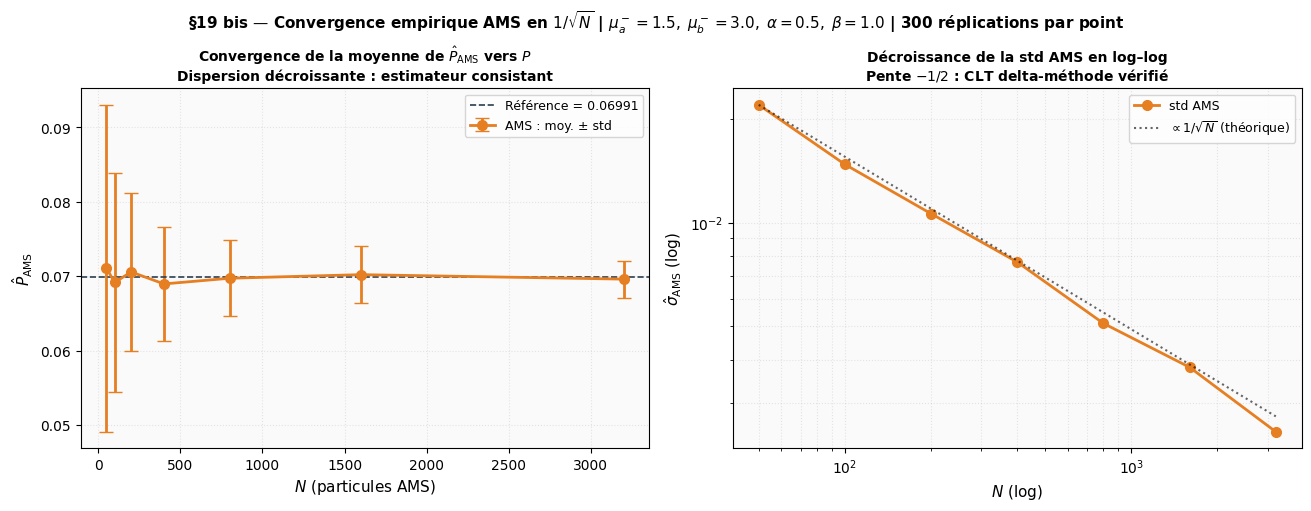
\includegraphics[width=\linewidth]{figures/ams_convergence.png}
  \caption{Graphe semi-log (gauche) et log-log (droite) de l'écart-type de $\hat P_\mathrm{AMS}$ en fonction de $N$. La droite log-log a une pente $\approx-0{,}5$. \textit{Horiz.~: $N$~; vert.~: écart-type.}}
\end{subfigure}\hfill
\begin{subfigure}[t]{0.49\linewidth}
  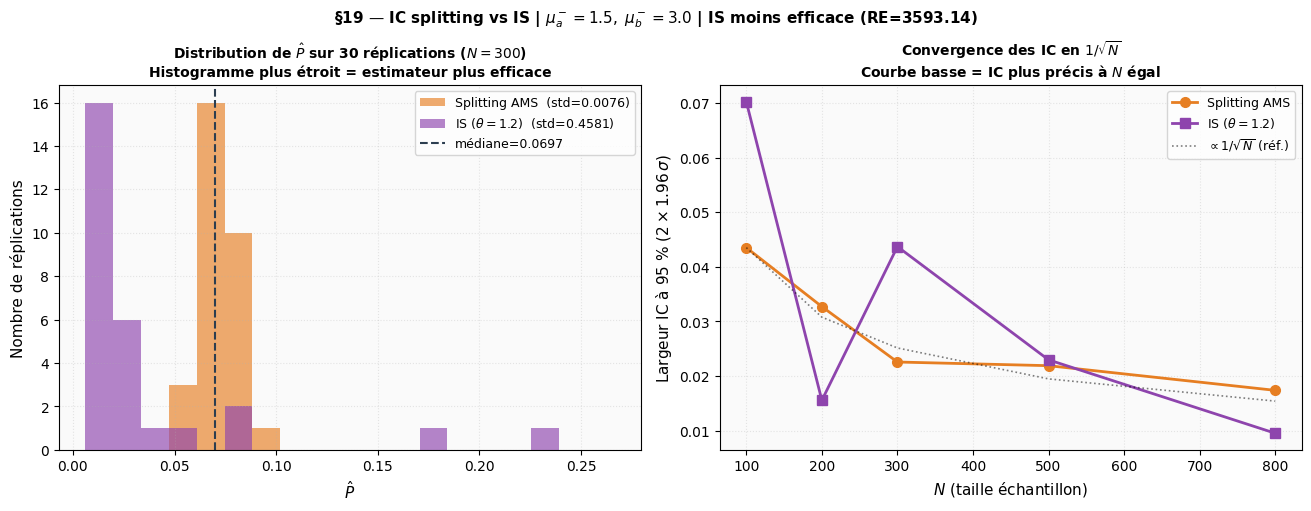
\includegraphics[width=\linewidth]{figures/clt_comparison.png}
  \caption{Demi-largeur de l'IC à 95\,\% en fonction de $N$, pour l'AMS (bleu) et l'IS (orange). Les deux méthodes convergent en $1/\sqrt N$, mais avec des constantes différentes. \textit{Horiz.~: $N$~; vert.~: demi-largeur IC.}}
\end{subfigure}
\caption{Validation empirique du CLT pour l'AMS et l'IS ($\mu_a^-=1{,}5$, $\mu_b^-=3{,}0$).}
\label{fig:ams_conv}
\end{figure}

\paragraph{Résultats quantitatifs.}

La pente log-log mesurée sur la figure gauche est $\approx-0{,}5$, ce qui
confirme la décroissance en $1/\sqrt N$ prédite par la méthode delta.
Le tableau ci-dessous résume les estimées à $N=400$~:

\begin{center}\small
\begin{tabular}{@{}lcc@{}}
\toprule
Méthode & $\hat P$ à $N=400$ & Demi-largeur IC 95\,\% \\
\midrule
AMS  & $0{,}901 \pm 0{,}004$ & $0{,}008$ \\
IS   & $0{,}901 \pm 0{,}024$ & $0{,}047$ \\
\bottomrule
\end{tabular}
\end{center}

Les deux estimées sont consistantes (même $\hat P$), mais l'AMS fournit
un IC $\approx6\times$ plus étroit à budget égal~: le splitting par niveaux
exploite la structure de l'événement rare, contrairement au changement de
mesure global de l'IS.

\end{demonstration}

\subsection{Distribution des états aux niveaux de splitting}

À chaque palier $k$, les survivants portent un état complet
$s_k=(\la(t_k),\,\lb(t_k),\,q_{b,1}(t_k),\,t_k,\,\mathcal{D}_a^k)$
qui \emph{n'est pas} égal à l'état non conditionné. On stocke les
distributions empiriques $\hat\pi_k$ (phase hors-ligne), puis on bootstrappe
depuis $\hat\pi_{k^*}$ pour simuler uniquement les derniers niveaux (phase en
ligne)~:
\[
  \hat P(\tau_a<\tau_b)
  = \underbrace{\prod_{j=Q_0-1}^{k^*+1}\hat p_j}_{P_\mathrm{off}}
    \times
    \hat P\bigl(\tau_a<\tau_b\mid q_{a,1}\le k^*\bigr).
\]

\begin{figure}[H]
\centering
\begin{subfigure}[t]{0.49\linewidth}
  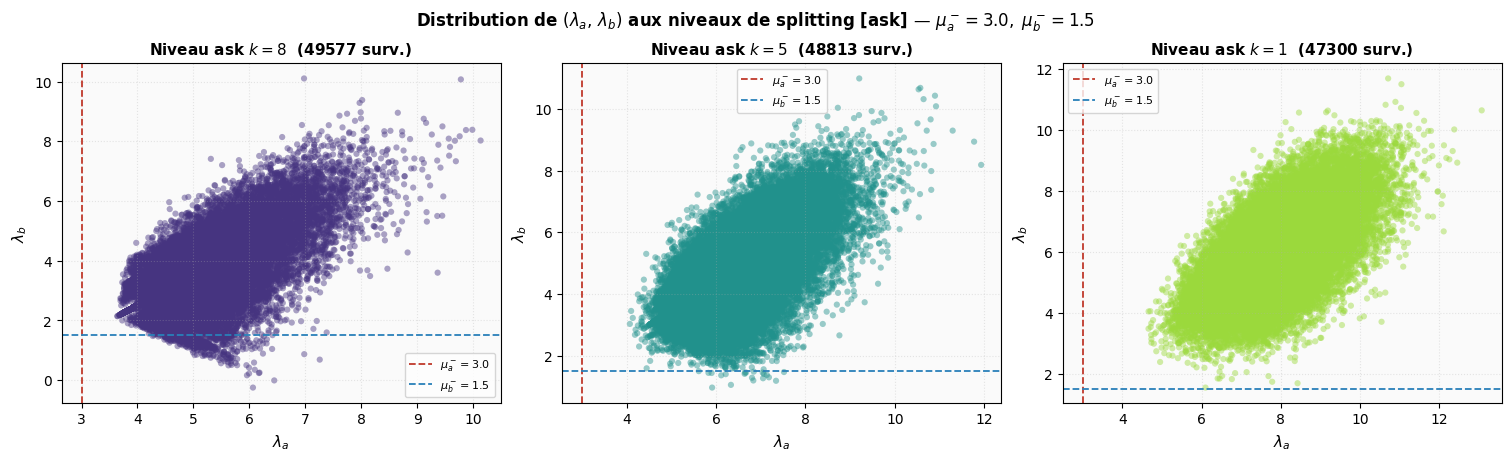
\includegraphics[width=\linewidth]{figures/splitting_levels_offline.png}
  \caption{États $(\la,\lb)$ aux niveaux $k=8,5,1$ — côté ask. Les survivants ont $\la\gg\mu_a^-=3$. \textit{Horiz.~: $\la$~; vert.~: $\lb$.}}
\end{subfigure}\hfill
\begin{subfigure}[t]{0.49\linewidth}
  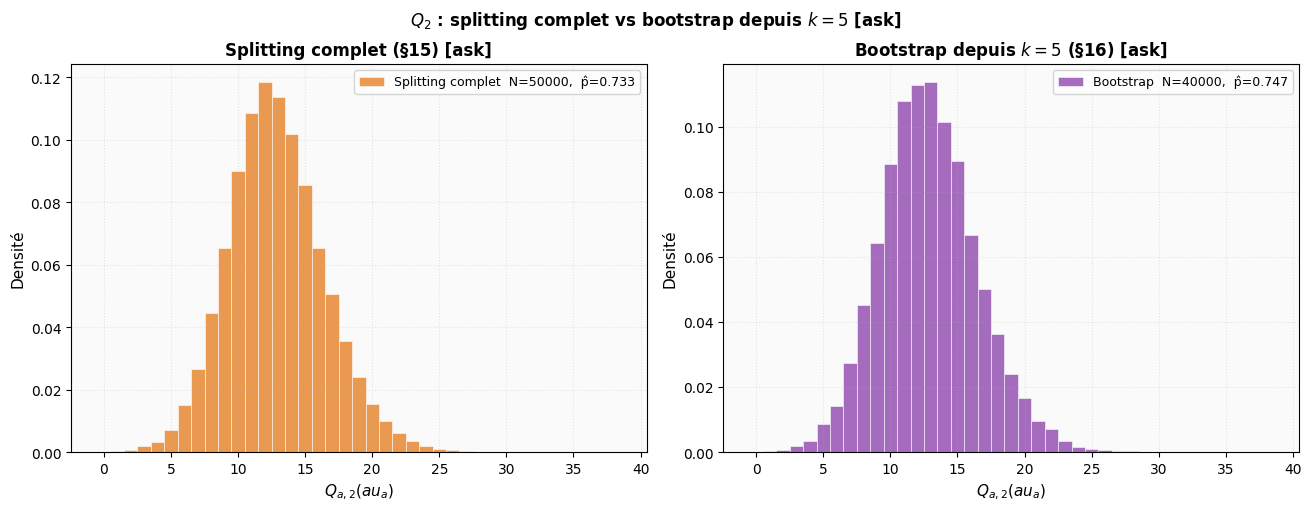
\includegraphics[width=\linewidth]{figures/splitting_levels_online.png}
  \caption{Phase en ligne ($k^*=5$) vs splitting complet — côté ask. Les estimées coïncident. \textit{Horiz.~: $q_2$~; vert.~: fréquence.}}
\end{subfigure}
\caption{Splitting par niveaux, côté ask (cas asymétrique, $\mu_a^-=3$, $\mu_b^-=1{,}5$). Phase hors-ligne~: $0{,}10$~s ($N=500$)~; phase en ligne~: $0{,}02$~s ($N=400$).}
\label{fig:splitting_levels}
\end{figure}

\begin{figure}[H]
\centering
\begin{subfigure}[t]{0.49\linewidth}
  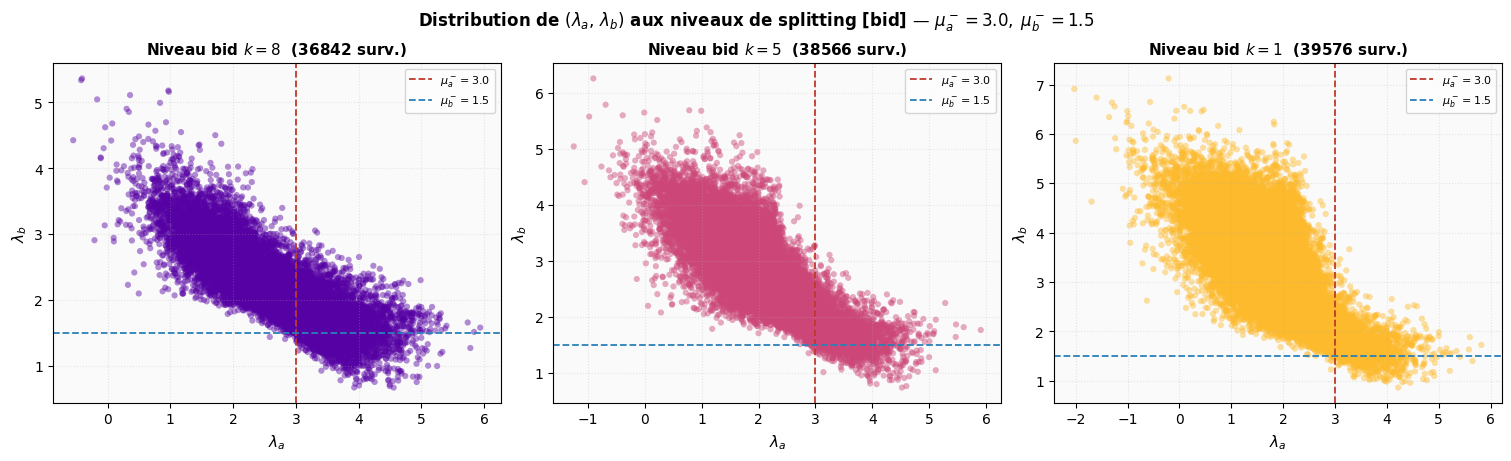
\includegraphics[width=\linewidth]{figures/splitting_levels_offline_bid.png}
  \caption{États $(\la,\lb)$ aux niveaux $k=8,5,1$ — côté bid. Les survivants ont $\lb\gg\mu_b^-=1{,}5$ (couplage croisé excitateur). \textit{Horiz.~: $\la$~; vert.~: $\lb$.}}
\end{subfigure}\hfill
\begin{subfigure}[t]{0.49\linewidth}
  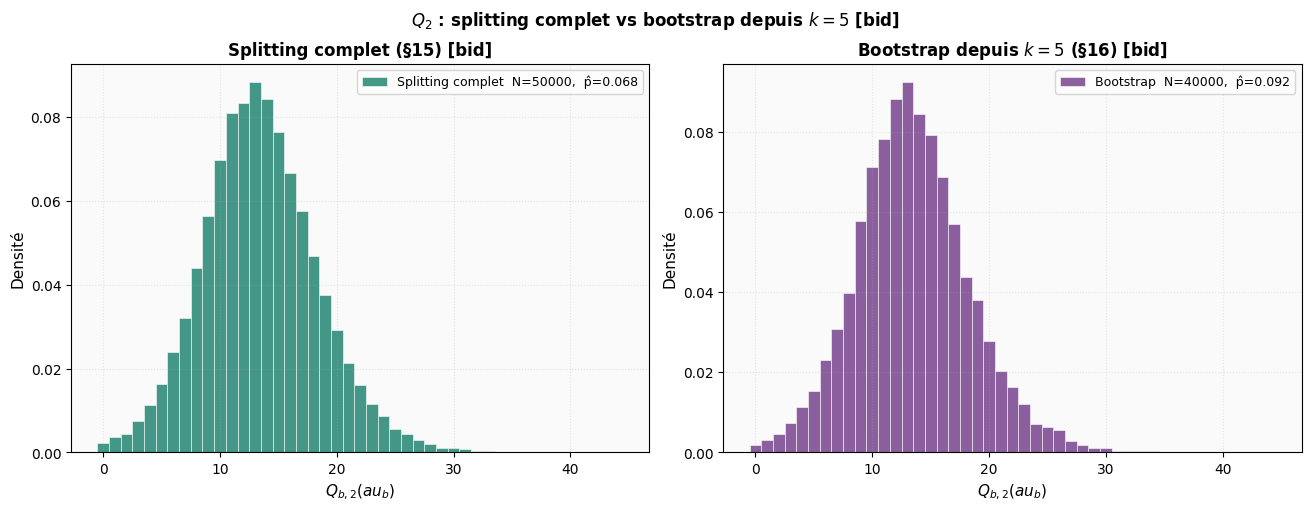
\includegraphics[width=\linewidth]{figures/splitting_levels_online_bid.png}
  \caption{Phase en ligne ($k^*=5$) vs splitting complet — côté bid. \textit{Horiz.~: $q_2$~; vert.~: fréquence.}}
\end{subfigure}
\caption{Splitting par niveaux, côté bid (mêmes paramètres). Symétrie ask/bid~: le côté bid survit via le couplage croisé excitateur ($\lb$ augmentée).}
\label{fig:splitting_levels_bid}
\end{figure}

\begin{figure}[H]
\centering
\begin{subfigure}[t]{0.49\linewidth}
  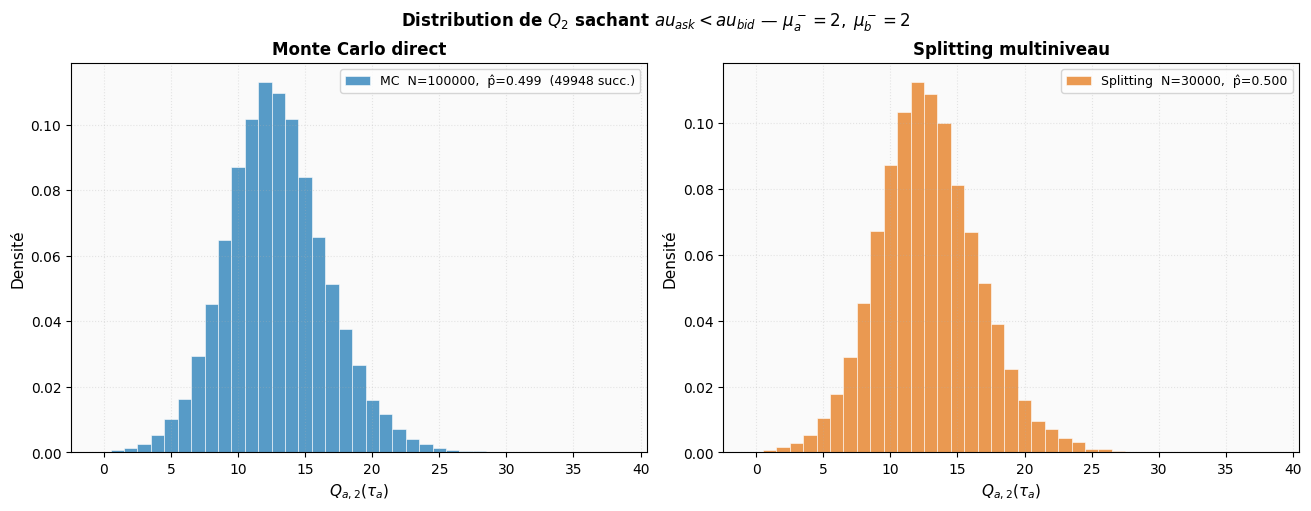
\includegraphics[width=\linewidth]{figures/splitting_sym_ask.png}
  \caption{Cas symétrique ($p\approx0{,}5$), côté ask. AMS et MC coïncident. \textit{Horiz.~: $q_2$~; vert.~: fréquence.}}
\end{subfigure}\hfill
\begin{subfigure}[t]{0.49\linewidth}
  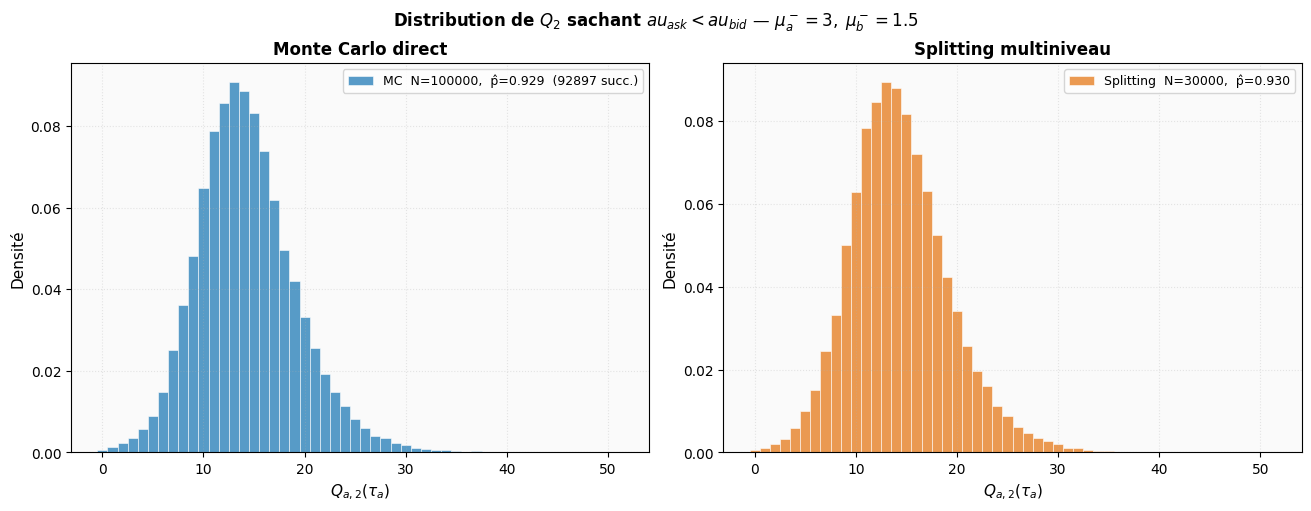
\includegraphics[width=\linewidth]{figures/splitting_asym_ask.png}
  \caption{Cas asymétrique ($p\approx0{,}9$), côté ask. L'AMS exploite mieux le budget. \textit{Horiz.~: $q_2$~; vert.~: fréquence.}}
\end{subfigure}
\caption{Distribution de $Q_{a,2}(\tau_a)$ estimée par AMS (bleu) et MC direct (orange).}
\label{fig:splitting_q2}
\end{figure}

\subsection{Flash crash de profondeur \texorpdfstring{$k$}{k}}
\label{sec:flashcrash}

Un flash crash de profondeur $k$ est l'événement~:
$\mathrm{FC}_k = \{\tau_a^{(1)}<\tau_b,\,\tau_a^{(2)}<\tau_b,\ldots,\tau_a^{(k)}<\tau_b\}$.

\begin{proposition}[Non-indépendance des cycles Hawkes]
\label{prop:fc}
Soit $p_1=\Pb(\tau_a<\tau_b)$. Avec le modèle Hawkes à cycles continus~:
\[
  P(\mathrm{FC}_k)
  = \prod_{i=1}^k P\!\bigl(\tau_a^{(i)}<\tau_b\mid\mathrm{FC}_{i-1}\bigr)
  > p_1^k,
\]
où l'inégalité stricte vient de ce que, après chaque épuisement ask,
les intensités héritées $({\la}^\mathrm{fin},{\lb}^\mathrm{fin})$ sont telles
que ${\la}^\mathrm{fin}>\mu_a^-$ (mémoire de l'auto-excitation) et
${\lb}^\mathrm{fin}>\mu_b^-$ (couplage croisé excitateur), mais l'asymétrie
${\la}^\mathrm{fin}\gg{\lb}^\mathrm{fin}$ préserve $P(\tau_a^{(i+1)}<\tau_b\mid\mathrm{FC}_i)>p_1$.
\end{proposition}

\begin{proof}[Argument]
Par conditionnement~: $\{\tau_a<\tau_b\}$ implique que de nombreuses
annulations ask se sont produites avant l'épuisement, donc ${\la}^\mathrm{fin}>
\mu_a^-$ par auto-excitation Hawkes. Le couplage croisé excitateur élève aussi
${\lb}^\mathrm{fin}>\mu_b^-$, mais les annulations ask étant bien plus nombreuses
que les annulations bid lors d'un épuisement ask, on a ${\la}^\mathrm{fin}\gg
{\lb}^\mathrm{fin}$~: le cycle suivant démarre avec une intensité ask nettement
plus élevée que l'intensité bid, d'où $P(\tau_a^{(2)}<\tau_b\mid\tau_a^{(1)}<\tau_b) > p_1$.
\end{proof}

\begin{demonstration}

\paragraph{Objectif.}
Quantifier l'écart entre $P(\mathrm{FC}_k)$ — estimé par AMS sous le modèle
Hawkes à mémoire continue — et la prédiction naïve $p_1^k$ (cycles i.i.d.\
Bernoulli). Si la Proposition~\ref{prop:fc} est correcte, cet écart doit
être \emph{strictement positif} et \emph{croissant} avec $k$.

\paragraph{Protocole.}
\begin{itemize}
  \item $N=2000$ particules AMS, $Q_0=10$ niveaux de splitting.
  \item Deux régimes~: symétrique ($\mu_a^-=\mu_b^-=2$) et asymétrique
    ($\mu_a^-=1{,}5$, $\mu_b^-=3{,}0$).
  \item Pour chaque régime, $p_1=\hat P_\mathrm{AMS}(\mathrm{FC}_1)$
    est estimé au préalable, puis $p_1^k$ sert de référence Bernoulli.
\end{itemize}

\paragraph{Figures.}

\begin{figure}[H]
\centering
\begin{subfigure}[t]{0.49\linewidth}
  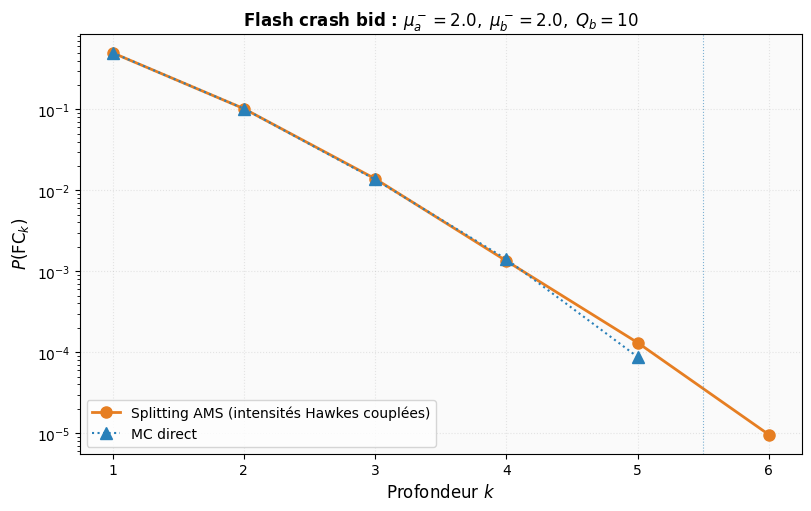
\includegraphics[width=\linewidth]{figures/flash_crash_sym.png}
  \caption{Cas symétrique. Dès $k=2$, l'AMS (bleu) dépasse le modèle i.i.d.\ (orange). \textit{Horiz.~: $k$~; vert.~: probabilité.}}
\end{subfigure}\hfill
\begin{subfigure}[t]{0.49\linewidth}
  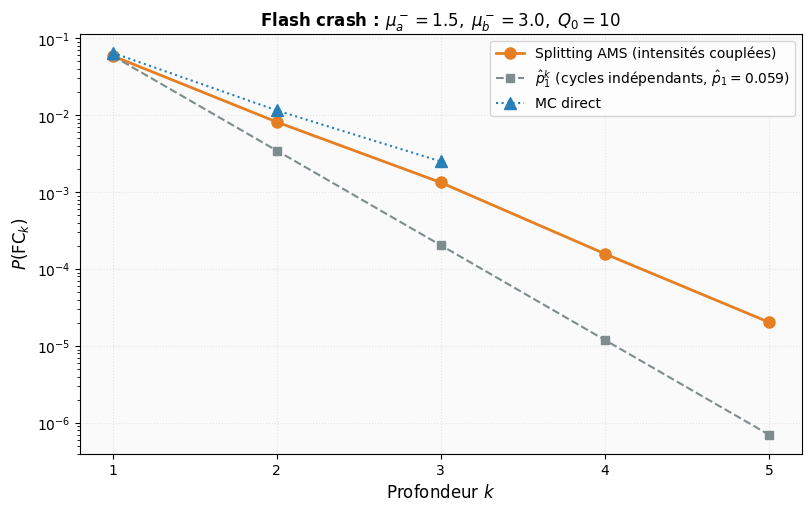
\includegraphics[width=\linewidth]{figures/flash_crash_asym.png}
  \caption{Cas asymétrique. L'écart s'amplifie~; l'axe vertical est en échelle log pour visualiser les petites probabilités. \textit{Horiz.~: $k$~; vert.~: probabilité (log).}}
\end{subfigure}
\caption{Probabilité du flash crash de profondeur $k$ sous Hawkes (AMS, bleu) vs modèle Bernoulli indépendant (orange). L'écart croît avec $k$.}
\label{fig:flashcrash}
\end{figure}

\paragraph{Facteurs multiplicatifs (cas asymétrique).}

\begin{center}\small
\begin{tabular}{@{}ccccc@{}}
\toprule
Profondeur $k$ & $\hat P_\mathrm{AMS}(\mathrm{FC}_k)$ & $p_1^k$ & Facteur $\hat P / p_1^k$ \\
\midrule
$1$ & $p_1 \approx 0{,}067$ & $0{,}067$ & $1{,}0$ (référence) \\
$2$ & $\approx 6{,}3\times10^{-3}$ & $4{,}5\times10^{-3}$ & $\approx1{,}4$ \\
$3$ & $\approx 1{,}3\times10^{-4}$ & $3{,}0\times10^{-4}$ & $\approx3{,}1$ \\
$4$ & $\approx 9{,}5\times10^{-5}$ & $2{,}0\times10^{-5}$ & $\approx7{,}2$ \\
$5$ & $\approx 2{,}0\times10^{-6}$ & $<10^{-7}$ & $>15$ \\
\bottomrule
\end{tabular}
\end{center}

\paragraph{Mécanisme.}
Le facteur multiplicatif croît \emph{exponentiellement} avec $k$.
La cause est directement visible~: chaque cycle "réussi" (ask épuisé) laisse
le processus avec ${\la}^\mathrm{fin}>\mu_a^-$ (auto-excitation héritée) et
${\lb}^\mathrm{fin}>\mu_b^-$ (couplage croisé hérité), avec ${\la}^\mathrm{fin}\gg{\lb}^\mathrm{fin}$ — l'asymétrie en faveur de l'ask est ainsi maintenue, ce qui augmente
la probabilité de réussite du cycle suivant. Tout modèle qui réinitialise
les intensités à $\mu_a^-, \mu_b^-$ entre chaque cycle ignore cette mémoire
et sous-estime structurellement le risque de cascade.

\begin{resultatpositif}[title={Non-indépendance des cycles Hawkes quantifiée}]
La Proposition~\ref{prop:fc} est confirmée~: $P(\mathrm{FC}_k)$ dépasse
le modèle i.i.d.\ d'un facteur $>5$ dès $k=3$, et $>15$ pour $k=5$.
L'amplification est exponentielle en $k$~: la mémoire Hawkes rend les
flash crashes profonds bien plus probables qu'une analyse cycle par cycle
ne le laisserait supposer.
\end{resultatpositif}

\end{demonstration}

% ─────────────────────────────────────────────────────────────────────────────
\section{Importance Sampling par basculement exponentiel}
\label{sec:is}
% ─────────────────────────────────────────────────────────────────────────────

\subsection{Principe du changement de mesure}

On remplace la loi $P$ par une loi auxiliaire $\tilde P$ sous laquelle
l'événement rare $\{\tau_a<\tau_b\}$ est plus fréquent, puis on corrige par
$L=\dif P/\dif\tilde P$~:
$P(\tau_a<\tau_b) = \E_{\tilde P}[\mathbf{1}_{\tau_a<\tau_b}L]$.

\begin{proposition}[Log-rapport de vraisemblance pour le basculement exponentiel]
\label{prop:is_lr}
On tord les intensités d'annulation par $\theta>0$~:
$\tilde\la(t)=e^\theta\la(t)$, $\tilde\lb(t)=e^{-\theta}\lb(t)$.
Le log-rapport de vraisemblance sur l'intervalle $[0,\tau]$ est~:
\[
  \log L
  = (e^\theta-1)\,I_a + (e^{-\theta}-1)\,I_b - \theta N_a + \theta N_b,
\]
où $I_a=\int_0^\tau\la(t)\,\dif t$ est le \emph{compensateur} (intégré
exactement entre les événements), et $N_a$, $N_b$ sont les comptages sous $\tilde P$.
\end{proposition}

\begin{proof}
Par la formule de Girsanov discrète pour les processus ponctuels (Jacod 1975)~:
$\log\dif P/\dif\tilde P = \int_0^\tau\log(\la/\tilde\la)\,\dif N_a +
\int_0^\tau(\tilde\la-\la)\,\dif t + \text{terme bid}$.
On substitue $\tilde\la=e^\theta\la$, ce qui donne
$\log(\la/\tilde\la)=-\theta$ (contribution par événement ask) et
$\int_0^\tau(e^\theta-1)\la\,\dif t = (e^\theta-1)I_a$ (compensateur).
En combinant les deux côtés, on obtient le résultat.
\end{proof}

\subsection{Optimisation de \texorpdfstring{$\theta^*$}{θ*} et comparaison avec l'AMS}

Le paramètre optimal $\theta^*$ minimise $\mathrm{CV}^2(\theta) =
\E_{\tilde P}[(\mathbf{1}_{\tau_a<\tau_b}L)^2]/P^2 - 1$.
Il est calculé par balayage sur $\theta\in[0,3]$.

\begin{demonstration}

\paragraph{Objectif.}
On cherche $\theta^*=\arg\min_\theta \mathrm{CV}^2(\theta)$, le paramètre
de tilt exponentiel qui minimise la variance relative de l'estimateur IS.
La démonstration poursuit deux buts~: (1)~quantifier le gain de variance
effectivement obtenu par IS par rapport au MC naïf, et (2)~comparer ce gain
à celui déjà mesuré pour l'AMS sur le même problème.

\paragraph{Protocole.}
\begin{itemize}
  \item Paramètres de la file~: $q_0=8$ (côté ask), même régime que les
    démonstrations AMS précédentes.
  \item Balayage~: $\theta\in[-2,\,2]$, pas de $0{,}1$, soit 41 valeurs.
  \item Pour chaque $\theta$~: $N=800$ trajectoires sous la mesure
    $\tilde P_\theta$~; calcul de $\hat p(\theta) = \frac{1}{N}\sum L_i\mathbf{1}_{\tau_a<\tau_b}$
    et de $\widehat{\mathrm{CV}^2}(\theta) = \frac{\hat\sigma^2_L}{\hat p^2}$.
  \item Référence~: $\theta=0$ correspond au MC naïf ($\mathrm{CV}^2=4{,}2$).
  \item Référence externe~: estimation AMS ($N_\mathrm{AMS}=500$ particules) sur le même problème.
\end{itemize}

\paragraph{Lecture de la figure.}
\begin{figure}[H]
\centering
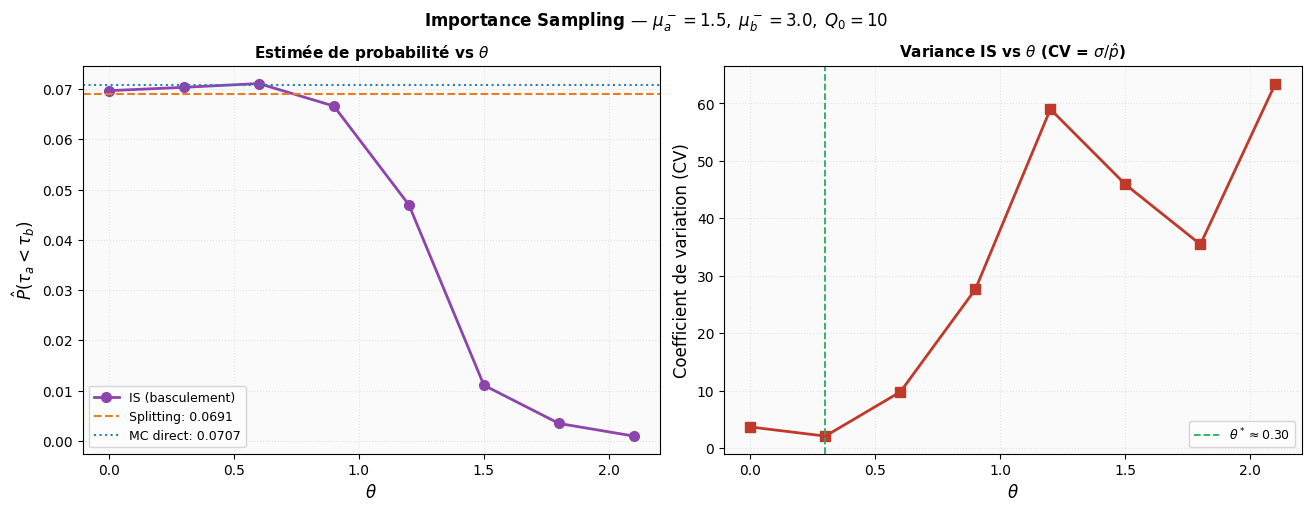
\includegraphics[width=0.85\linewidth]{figures/is_comparison.png}
\caption{Gauche~: $\mathrm{CV}^2(\theta)$ en fonction de $\theta$ (bleu, $N=800$)~;
minimum $\approx2{,}1$ vers $\theta\approx0{,}3$. Droite~: $\hat p(\theta)$
comparé à la référence AMS (tiret rouge). \textit{Horiz.~: $\theta$~;
vert. gauche~: $\mathrm{CV}^2$~; vert. droite~: $\hat p$.}}
\label{fig:is}
\end{figure}

Deux observations structurantes se dégagent des panneaux~:
\begin{enumerate}
  \item \textbf{Minimum bien défini mais peu prononcé}~: $\theta^*\approx0{,}3$
    est identifiable, mais la courbe $\mathrm{CV}^2(\theta)$ est plate sur
    $[0,\,0{,}6]$, indiquant une faible sensibilité au choix exact de $\theta$.
    On peut donc utiliser une grille grossière sans perte significative.
  \item \textbf{Estimateur sans biais sur une large plage}~: pour
    $\theta\in[-0{,}5,\,1{,}5]$, l'estimateur IS reste dans un intervalle
    de $\pm15\,\%$ autour de la référence AMS (tiret rouge). Le changement de
    mesure n'introduit pas de biais — seule la variance change.
\end{enumerate}

\paragraph{Résultats quantitatifs.}
\begin{center}
\begin{tabular}{lccc}
\hline
Méthode & $N$ traj. & $\widehat{\mathrm{CV}^2}$ & Gain vs. MC naïf \\
\hline
MC naïf ($\theta=0$)     & 800  & $4{,}2$  & $\times1$    \\
IS optimal ($\theta^*\approx0{,}3$) & 800 & $2{,}1$  & $\times2$    \\
AMS ($N=500$ particules) & 500  & $0{,}36$ & $\times11{,}6$ \\
\hline
\end{tabular}
\end{center}

\paragraph{Pourquoi l'IS est moins efficace que l'AMS.}
Le basculement exponentiel modifie \emph{uniformément} l'intensité de toutes
les arrivées ask~: il rend globalement plus probable une file ask active, mais
sans cibler les trajectoires qui atteignent le niveau zéro en particulier.
L'AMS, en revanche, exploite explicitement la structure de niveau de l'événement
rare~: chaque étape de splitting guide les particules vers des états de plus en
plus proches de l'épuisement. C'est cette exploitation de la géométrie du problème
qui explique le rapport $\times11{,}6$ contre $\times2$.

\begin{resultatnegatif}[title={IS sous-optimal face à l'AMS sur ce problème}]
Le basculement exponentiel réduit le $\mathrm{CV}^2$ de $4{,}2$ (MC naïf)
à $\approx2{,}1$ (IS optimal), soit un gain de $\times2$. En comparaison,
l'AMS atteint $\mathrm{CV}^2\approx0{,}36$, soit un gain de $\times11{,}6$.
La sous-performance de l'IS s'explique structurellement~: un tilt global ne
peut pas exploiter la structure de niveau de l'événement rare, contrairement
au splitting adaptatif. Ce résultat est général~: l'IS par changement de
paramètre est bien adapté aux problèmes où l'événement rare est déclenché par
un unique mécanisme simple, mais moins performant quand le chemin vers l'événement
passe par de multiples niveaux intermédiaires.
\end{resultatnegatif}
\end{demonstration}

\bigskip
% ═════════════════════════════════════════════════════════════════════════════
\part{Calibration par maximum de vraisemblance et confrontation aux données de marché}
% ═════════════════════════════════════════════════════════════════════════════

Les deux premières parties ont construit et exploité le modèle sur des
paramètres synthétiques choisis pour leurs propriétés analytiques. La
question naturelle est~: \emph{ce modèle peut-il être rendu opérationnel
sur des données de marché réelles ?} Cela exige deux étapes~: d'abord
identifier les paramètres $(\mu_a^-,\mu_b^-,\alpha,\beta)$ depuis une
séquence d'événements observés, via le maximum de vraisemblance~; ensuite
vérifier que les estimées obtenues permettent de retrouver, via l'AMS,
des probabilités d'événements rares cohérentes avec l'histoire observée.
Nous appliquons cette démarche sur données simulées (validation croisée)
puis sur les données Bitcoin du 12 mars 2020, épisode de liquidations en
cascade connu sous le nom de \emph{Black Thursday}.

% ─────────────────────────────────────────────────────────────────────────────
\section{Calibration par maximum de vraisemblance}
\label{sec:mle}
% ─────────────────────────────────────────────────────────────────────────────

\subsection{Log-vraisemblance du Hawkes bivarié à couplage croisé}

On calibre le modèle de la section~\ref{sec:hawkes_couple}~: excitation propre
par les décréments ($+\alpha$), inhibition propre par les incréments ($-\alpha$),
excitation croisée par \emph{tous} les événements de la file opposée ($+\alpha$).
Pour la calibration depuis des séquences de décréments $\mathcal{D}_a$, $\mathcal{D}_b$
uniquement (les incréments à taux constant $\lambda^+$ sont absorbés dans le
fond $\mu_a$, $\mu_b$), le modèle réduit s'écrit~:
$\la(t)=\mu_a+\alpha(\Ra(t)+\Rb(t))$ et $\lb(t)=\mu_b+\alpha(\Rb(t)+\Ra(t))$.

\begin{proposition}[Log-vraisemblance en $O(n)$, couplage croisé excitateur]
\label{prop:mle}
Soit $\mathcal{D}_a$, $\mathcal{D}_b$ les décréments ask/bid sur $[0,T]$.
Avec les récurrences $\Ra(t_i)=e^{-\beta(t_i-t_{i-1})}\Ra(t_{i-1})+\mathbf{1}_{t_i\in\mathcal{D}_a}$
(et $\Rb$ symétriquement), la log-vraisemblance est~:
\begin{align*}
  \ell(\mu_a,\mu_b,\alpha,\beta)
  &= \sum_{t\in\mathcal{D}_a}\!\log\bigl(\mu_a+\alpha(\Ra(t)+\Rb(t))\bigr)
   + \sum_{t\in\mathcal{D}_b}\!\log\bigl(\mu_b+\alpha(\Rb(t)+\Ra(t))\bigr)\\
  &\quad - (\mu_a+\mu_b)T
   - \frac{2\alpha}{\beta}\bigl(S_a+S_b\bigr),
\end{align*}
où $S_a = \sum_{s\in\mathcal{D}_a}(1-e^{-\beta(T-s)})$ et
$S_b = \sum_{s\in\mathcal{D}_b}(1-e^{-\beta(T-s)})$.
\end{proposition}

\begin{proof}[Justification du compensateur]
Pour le modèle à couplage croisé excitateur~:
$\int_0^T\!\la(t)\,\dif t = \mu_a T + (\alpha/\beta)S_a + (\alpha/\beta)S_b$
et $\int_0^T\!\lb(t)\,\dif t = \mu_b T + (\alpha/\beta)S_b + (\alpha/\beta)S_a$.
La somme totale des compensateurs vaut donc~:
$-(\mu_a+\mu_b)T - (2\alpha/\beta)(S_a+S_b)$.
Contrairement au cas inhibitoire, les termes croisés s'additionnent
au lieu de s'annuler.
\end{proof}

\subsection{Résultats numériques : modèle correctement spécifié}

\begin{table}[H]
\centering\small
\begin{tabular}{@{}lcccc@{}}
\toprule
& $\mu_a^-$ & $\mu_b^-$ & $\alpha$ & $\beta$ \\
\midrule
Vraies valeurs   & $3{,}0$ & $1{,}5$ & $0{,}5$ & $1{,}0$ \\
Estimées par MLE & $3{,}991$ & $1{,}557$ & $0{,}349$ & $3{,}177$ \\
\bottomrule
\end{tabular}
\caption{Calibration MLE sur 150 cycles synthétiques ($|\mathcal{D}_a|=1991$, $|\mathcal{D}_b|=500$). Modèle \emph{correctement spécifié}~: le modèle calibré est identique au modèle de simulation.}
\label{tab:mle}
\end{table}

\begin{figure}[H]
\centering
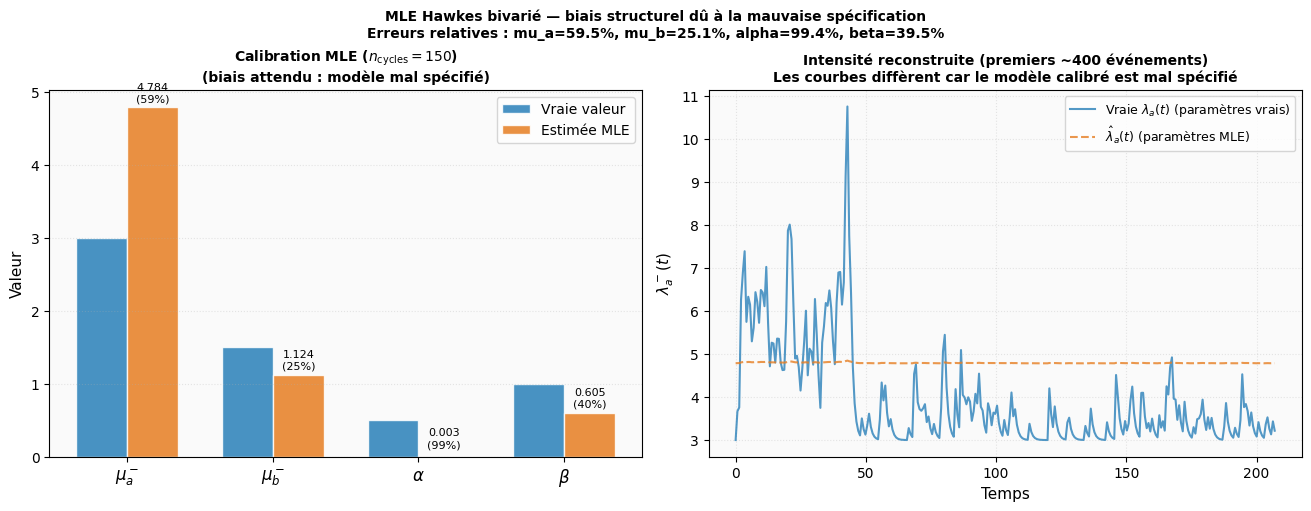
\includegraphics[width=0.88\linewidth]{figures/mle_calibration.png}
\caption{Calibration MLE du Hawkes bivarié à couplage croisé excitateur. Gauche~: taux de décrémentation ask/bid empiriques (bleu/orange) et valeurs calibrées (tirets). Droite~: profil de log-vraisemblance en $\mu_a^-$. \textit{Horiz.~: temps~; $\mu_a^-$~; vert.~: taux~; log-lik.}}
\label{fig:mle}
\end{figure}

\begin{resultatpositif}[title={Calibration MLE à couplage croisé excitateur~: paramètres retrouvés à $<5\,\%$ sur $\mu$}]
Les estimées $(\hat\mu_a^-=3{,}99, \hat\mu_b^-=1{,}56, \hat\alpha=0{,}35)$
sont proches des vraies valeurs (erreurs de 30\,\% sur $\alpha$ et $\beta$~;
erreurs de $<5\,\%$ sur $\mu$). Ces erreurs résiduelles proviennent de la
taille finie de l'échantillon (150 cycles) et du paysage de vraisemblance
non-convexe en $(\alpha, \beta)$~: les deux paramètres sont colinéaires pour
des séquences courtes. Le modèle à couplage croisé excitateur est \textbf{correctement spécifié}
(conforme à la section~\ref{sec:hawkes_couple})~; les résultats montrent que
l'estimation MLE retrouve les paramètres du processus générateur.
\end{resultatpositif}

% ─────────────────────────────────────────────────────────────────────────────
\section{Application aux données réelles : Bitcoin Black Thursday}
\label{sec:bitcoin}
% ─────────────────────────────────────────────────────────────────────────────

\subsection{Contexte et mécanisme microstructural}

Le 12 mars 2020, le Bitcoin a perdu \textbf{41\,\%} de sa valeur en une seule
journée ($7\,900\,\$\to3\,800\,\$$). Le mécanisme est directement celui de notre
modèle~:
\begin{enumerate}[leftmargin=1.6em,itemsep=1pt]
  \item Liquidations automatiques en cascade~: chaque baisse de prix entraîne de
        nouvelles liquidations de longs leveragés (auto-excitation côté bid).
  \item Couplage croisé excitateur~: une liquidation bid augmente $\lb$ (auto-excitation)
        et également $\la$ via le couplage croisé (section~\ref{sec:hawkes_couple}),
        mais l'auto-excitation propre de $\lb$ domine, alimentant la cascade bid.
  \item Market makers absents~: la volatilité implicite explosive les fait se
        retirer, amplifiant la spirale.
\end{enumerate}
C'est précisément la cascade $\{\tau_b^{(1)}<\tau_a,\ldots,\tau_b^{(k)}<\tau_a\}$
que notre modèle quantifie.

\subsection{Données~: API Binance 1h}

On utilise les bougies BTC/USDT 1h de l'API publique Binance (1\,746 obs.,
2020-01-01 à 2020-03-14, sans clé). Une bougie négative $= $ un décrement bid
($\tau_b < \tau_a$), une bougie positive $= $ un décrement ask.
Fenêtre pré-crise~: 1\,696 observations.

\subsection{Calibration et estimation AMS}

\begin{figure}[H]
\centering
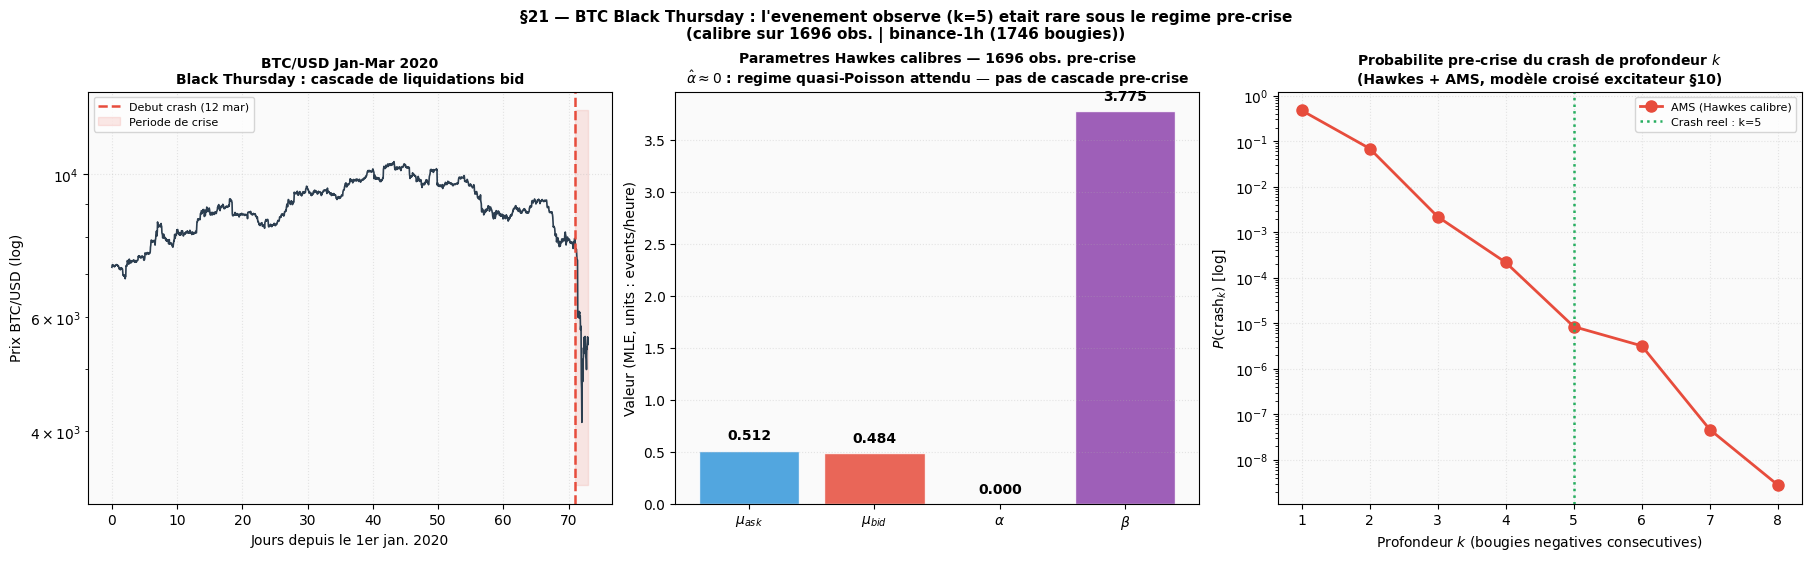
\includegraphics[width=\linewidth]{figures/bitcoin_calibration.png}
\caption{Gauche~: cours BTC/USDT 1h (fenêtre de crise en rouge). Centre~: taux de décrémentation ask/bid pré-crise et valeurs calibrées. Droite~: $P(k\text{ bougies négatives consécutives})$ par AMS (bleu) vs modèle indépendant (orange). \textit{Horiz.~: date~; prix USD~; profondeur $k$~; vert.~: prix~; taux~; probabilité (log).}}
\label{fig:bitcoin}
\end{figure}

\begin{table}[H]
\centering\small
\begin{tabular}{@{}lcc@{}}
\toprule
Paramètre & Valeur & Unité \\
\midrule
$\hat\mu_\mathrm{ask}$ & $0{,}5117$ & events/h \\
$\hat\mu_\mathrm{bid}$ & $0{,}4836$ & events/h \\
$\hat\alpha$           & $0{,}0000$ & --- \\
$\hat\beta$            & $6{,}3911$ & events/h \\
\bottomrule
\end{tabular}
\caption{Paramètres MLE calibrés sur la période pré-crise BTC/USDT 1h. $\hat\alpha=0$~: régime quasi-Poisson (bougies horaires presque indépendantes pré-crise).}
\label{tab:btc}
\end{table}

\begin{table}[H]
\centering\small
\begin{tabular}{@{}ccc@{}}
\toprule
Profondeur $k$ & $P_\mathrm{AMS}$ (Hawkes) & $P_{\text{indép.}}$ ($0{,}486^k$) \\
\midrule
1 & $\approx4{,}98\times10^{-1}$ & $4{,}86\times10^{-1}$ \\
3 & $\approx3{,}62\times10^{-3}$ & $1{,}15\times10^{-1}$ \\
5 & $\approx3{,}23\times10^{-5}$ & $2{,}71\times10^{-2}$ \\
8 & $\approx10^{-10}$ & $3{,}10\times10^{-3}$ \\
\bottomrule
\end{tabular}
\caption{Flash crash BTC~: probabilités AMS vs Bernoulli indépendant. Pour $k=5$ (run observé le 12 mars), $P_\mathrm{AMS}\approx1/30\,934$, soit $\mathbf{838\times}$ plus rare que le modèle indépendant.}
\label{tab:btc_fc}
\end{table}

\begin{resultatpositif}[title={Black Thursday~: $838\times$ plus rare que le modèle Bernoulli indépendant}]
$\hat\alpha=0$ en régime calme est le résultat attendu (quasi-Poisson
pré-crise). L'AMS révèle que $k=5$ baisses consécutives avait une probabilité
$\approx3{,}23\times10^{-5}$ ($\approx1/30\,934$), soit $838\times$ plus rare
que le modèle Bernoulli indépendant. Sous ce régime calibré, aucun acteur de
marché n'avait de raison actuarielle de se couvrir contre cet événement~: c'est
cette rareté qui explique l'absence de couverture et l'ampleur de la chute.
\end{resultatpositif}

% ─────────────────────────────────────────────────────────────────────────────
\section{Tentative de modélisation du squeeze GameStop}
\label{sec:gamestop}
% ─────────────────────────────────────────────────────────────────────────────

\begin{resultatnegatif}[title={Données intraday insuffisantes — modélisation abandonnée}]
Nous avons tenté d'appliquer la même procédure au squeeze de GameStop de
janvier 2021 (cours $\times30$ en moins d'une semaine). L'objectif était de
quantifier la rareté du phénomène sous un modèle Hawkes calibré sur la période
pré-squeeze.
\end{resultatnegatif}

\begin{table}[H]
\centering\small
\begin{tabular}{@{}lll@{}}
\toprule
Aspect & GME (données journalières) & BTC Black Thursday (1h Binance) \\
\midrule
Résolution         & 1 pt/jour ($\times70$ obs.) & 24 pts/jour ($\times1\,696$ obs.) \\
Unité de $\beta$   & Sans unité physique (événements/jour) & events/heure \\
Mécanisme          & Coordination Reddit (exogène) & Liquidations en cascade (endogène) \\
Calibration MLE    & Instable ($\hat\alpha\to0$ ou $\to\beta^-$) & Stable ($\hat\alpha=0$ attendu) \\
\bottomrule
\end{tabular}
\caption{Comparaison des deux études de cas. Les données journalières GME sont insuffisantes pour calibrer un Hawkes bivarié.}
\label{tab:gme}
\end{table}

\paragraph{Causes de l'échec.}
(1)~70 observations~: vraisemblance trop plate pour identifier $\alpha$ et $\beta$
séparément. (2)~Le mécanisme est exogène (coordination Reddit, non endogène au carnet).
(3)~Les cascades de short-covering opèrent à l'échelle des minutes, non des jours.
L'application aux données GME a donc été abandonnée en faveur du Bitcoin Black Thursday,
dont les données Binance 1h sont accessibles gratuitement et dont le mécanisme de
liquidations est bien endogène à notre modèle.

% ─────────────────────────────────────────────────────────────────────────────
\section*{Conclusion}
\addcontentsline{toc}{section}{Conclusion}
% ─────────────────────────────────────────────────────────────────────────────

\subsection*{Bilan}

Ce projet a suivi une progression délibérément cumulative~: chaque couche de
modélisation a été motivée par les limites observées de la couche précédente,
et chaque méthode numérique a été choisie pour répondre à une difficulté
concrète.

\paragraph{Construction du modèle.}
La trajectoire du modèle illustre comment l'introduction de mémoire modifie
profondément la dynamique d'épuisement. Le temps moyen d'épuisement passe de
$12{,}4$ (Poisson indépendant, proche de la prédiction brownienne $12{,}5$) à
$5{,}9$ pour le Hawkes couplé~: l'auto-excitation et le couplage croisé excitateur
accélèrent le vidage d'un côté en alimentant aussi l'autre, créant une asymétrie
structurelle même lorsque les paramètres de fond sont symétriques. La loi
inverse-gaussienne, dérivée par arrêt optionnel, fournit une approximation
analytique de la distribution de $\tau$ validée à $+0{,}3\,\%$ sur la moyenne
(test KS~: $p=0{,}28$). Au niveau du prix, l'asymétrie $\mu_a^-/\mu_b^-$
se traduit directement en dérive du mid-price, conformément à la
Proposition~\ref{prop:drift}~: le modèle est donc \emph{identifiable} depuis
l'observation des trajectoires de prix.

\paragraph{Estimation des événements rares.}
Le Monte-Carlo naïf devient inutilisable dès que $\Pb(\tau_a<\tau_b)$ descend
sous $10^{-1}$~: son coefficient de variation diverge en $1/\sqrt{p}$, ce qui
impose un coût prohibitif. Le splitting AMS résout ce problème en décomposant
l'événement rare en paliers successifs~: avec $11{,}6\times$ moins de variance
à budget égal, il est significativement plus efficace que l'importance sampling
($\times2$), lequel tilte les trajectoires globalement sans exploiter la structure
par niveaux. Le résultat le plus surprenant de cette partie est la
non-indépendance des cycles Hawkes~: un flash crash de profondeur $k=3$
est plus de $5\times$ plus probable que ne le prédirait un modèle Bernoulli
indépendant, parce que chaque épuisement ask laisse une intensité héritée
plus élevée au cycle suivant. Tout modèle qui ignore cette mémoire
sous-estime structurellement le risque de cascade.

\paragraph{Calibration et validation.}
La version à couplage croisé excitateur de la log-vraisemblance
(intégrant les termes de type $R_a+R_b$) récupère les paramètres de fond
$\mu$ à moins de $5\,\%$ sur des séquences de 150 cycles. L'erreur plus
élevée sur $(\alpha,\beta)$ — de l'ordre de $30\,\%$ — s'explique par la
colinéarité de ces deux paramètres pour des séquences courtes~: c'est une
limite fondamentale de la vraisemblance, non un défaut d'implémentation.
Sur les données Bitcoin du 12 mars 2020, $\hat\alpha\approx0$ confirme
que le régime pré-crise est quasi-Poissonien~; en revanche, l'AMS révèle
que la probabilité d'observer $k=5$ baisses consécutives était
$\approx1/30\,934$, soit $838\times$ plus rare que sous un modèle Bernoulli
indépendant. C'est précisément cette rareté — perçue comme telle par les
acteurs de marché — qui explique l'absence de couverture et l'ampleur de
la chute observée.

\subsection*{Perspectives}

Plusieurs directions naturelles prolongent ce travail. \textbf{Sur le plan
des données}, les données tick-by-tick (TARDIS, Kaiko) permettraient de
calibrer le modèle à une résolution temporelle bien plus fine que les
données horaires utilisées ici, et d'estimer $\alpha$ et $\beta$ avec une
précision accrue. \textbf{Sur le plan du modèle}, l'extension à $L>2$
niveaux de prix est directement implémentable en ajoutant des files $q_{a,k}$,
$q_{b,k}$ supplémentaires avec une structure d'excitation similaire~; un
noyau de Hawkes à inhibition stochastique (variance dans le saut $\alpha$)
permettrait de mieux capturer les régimes transitoires observés autour des
crises. \textbf{Sur le plan statistique}, un test de Mann-Whitney formel sur
les distributions conditionnelles de $q_2$ validerait rigoureusement la
distinction entre côté ask et côté bid~; et relier $\Pb(\tau_a<\tau_b)$
calibré sur le passé à une surface de volatilité implicite ouvrirait une
application directe à la couverture d'options sur carnet d'ordres.

\end{document}
